% !Mode:: "TeX:UTF-8"
%%  本模板推荐以下方式编译:
%%     1. PDFLaTeX[推荐]
%%     2. xelatex [含中文推荐]
%%  注意:
%%  1. 文件默认的编码为 UTF-8 对于windows,请选用支持UTF-8编码的编辑器。
%%   2. 若是模板有什么问题,请及时与我们取得联系,Email:latexstudio@qq.com。
%%   3. 可以到  https://ask.latexstudio.net 提问
%%   4. 请安装 最新版本的 TeXLive 地址:
%%   http://mirrors.ctan.org/systems/texlive/Images/texlive.iso

\documentclass{apmcmthesis}
\usepackage{indentfirst}
\usepackage{url}
\usepackage{float} %设置图片浮动位置的宏包
\usepackage{graphicx} %插入图片的宏包
\usepackage{subfigure} %插入多图时用子图显示的宏包
%%%%%%%%%%%%填写相关信息%%%%%%%%%%%%%%%%%%%%%%%%%%
\tihao{B}                            %选题
\baominghao{24212061}                 %参赛编号
\begin{document}

\pagestyle{frontmatterstyle}

\begin{abstract}
	
To address issues such as the large spatial footprint and safety hazards of separate devices such as air conditioners, air purifiers, and humidifiers, this study applies genetic algorithms to optimize the integration of these three functionalities into a single product.

For Problem 1, the optimal dimensions of an air conditioner (radius: 0.25 m, height: 0.5 m) were determined using a genetic algorithm implemented in Python, converging after 50 iterations. A heat conduction model was established based on fundamental physical principles and solved using the finite difference method to capture the variation of indoor temperature over time and space. Numerical simulations conducted via ANSYS Fluent validated the air conditioner's design as optimal.

For Problem 2, a genetic algorithm was used to optimize the design of an air purifier, yielding dimensions of radius 0.48 m and height 1.9 m. A gas concentration variation model based on Fick's Second Law simulated pollutant removal during operation, confirming the effectiveness of this design.

For Problem 3, particle swarm optimization (PSO), a method with faster convergence, was applied to optimize the humidifier's design. After 50 iterations, the optimal dimensions (radius: 0.18 m, height: 1 m) were determined. Using principles similar to those in Problem 2, simulations verified the humidifier's performance.

Finally, for Problem 4, a genetic algorithm combined the results of the first three problems to optimize the integration of the three functionalities, resulting in a cylindrical product with a radius of 0.25 m and a height of 0.4807 m.


\keywords{ANSYS Fluent\quad  Genetic Algorithm\quad  Particle Swarm Optimization\quad  Aerodynamics\quad Laplace Operator}
\end{abstract}



\newpage
%目录
\tableofcontents


\newpage
\pagestyle{mainmatterstyle}
\setcounter{page}{1}
\section{Introduction}

\subsection{ Background Analysis}
As technology evolves, the demand for enhanced living standards grows. The increasing use of devices like air conditioners, humidifiers, and air purifiers has introduced challenges such as the need for multiple power sources and excessive wiring, raising safety concerns and risks of electrical overload. To address these issues, a three-in-one device integrating air conditioning, humidifying, and air purification functions is proposed, offering a streamlined and efficient solution.

\subsection{Restatement of the Problem}
As living standards rise, integrated devices combining air conditioning, purification, and humidification functions are increasingly valued. This study focuses on market analysis and mathematical modeling to optimize the design of such a product.

Problem 1: Analyze critical factors such as placement, number, and location of air vents, as well as airflow direction, angle, wind speed, and volume. Simulate the indoor temperature distribution over time under summer and winter conditions. Based on the simulation results, determine the optimal shape and dimensions for enhanced performance.

Problem 2: Maximize the air purifier's efficiency by analyzing how its shape impacts purification performance. Develop an optimization model to identify the optimal design for achieving the best purification effect.

Problem 3: Enhance the humidifier’s performance by examining how its shape affects humidification. Develop and evaluate a model that considers these factors to design the optimal shape and dimensions.

Problem 4: Design a high-efficiency three-in-one product that integrates the functionalities of an air conditioner, air purifier, and humidifier. Combine the models from the first three problems to achieve maximum energy efficiency, comfort, purification, and humidification effects.





\section{Analysis of Individual Problems}
\subsection{ Air Conditioner Optimization}
To design the optimal air conditioner, analyze the effects of placement, air vent location and number, airflow direction and angle, wind speed, and volume on performance. Consider variations in indoor temperature during summer and winter conditions. Use a genetic algorithm to optimize the air conditioner's shape, applying the explicit finite difference method to analyze the indoor temperature field. ANSYS Fluent simulations validate the optimized design.


\subsection{Air Purifier Optimization}
For the air purifier, assess how various shapes impact purification efficiency. A genetic algorithm is used to establish a model for optimizing its shape, utilizing Fick's Second Law to examine the variation in indoor pollutant concentrations. The resulting data is used to define the optimal design.

\subsection{Humidifier Optimization}
To improve humidification efficiency, examine the impact of shape using a particle swarm optimization algorithm. Employ Fick's Second Law to study indoor humidity variations and assess how humidification effectiveness evolves over time, leading to the optimal humidifier design.




\subsection{Three-in-One Product Optimization}
Integrate the designs from the first three problems using a genetic algorithm to simulate the combined model. The goal is to maximize energy efficiency, comfort, purification, and humidification in a single product.


\section{Model Assumptions}

1.Indoor temperature variations are influenced only by external temperature, air conditioner outlet temperature, and airflow velocity. Feedback effects from wall temperatures are ignored.\\

2.Airflow velocities at the inlets and outlets of all devices are constant.

3.Indoor air is treated as an ideal gas with physical properties invariant to environmental changes.
\section{Symbol Definitions}

	\begin{table}[h]
		\centering
		\caption{Symbols and their meanings with units}
		\label{tab:symbols}
		\begin{tabular}{lll}
			\toprule
			\textbf{Symbol} & \textbf{Meaning} & \textbf{Unit} \\
			\midrule
			$w(x,y,z)$ & Weight at a spatial point & - \\
			$\Delta t$ & Time step & s \\
			CARD & Purification efficiency & - \\
			$T_n$ & Temperature at time step $n$ & K \\
			$T_{n+1}$ & Temperature at time step $n+1$ & K \\
			$C_n$ & Concentration at time step $n$ & $\frac{g}{m^3}$ \\
			$C_{n+1}$ & Concentration at time step $n+1$ & $\frac{g}{m^3}$ \\
			$H_n$ & Humidity at time step $n$ & $\frac{g}{m^3}$ \\
			$H_{n+1}$ & Humidity at time step $n+1$ & $\frac{g}{m^3}$ \\
			\bottomrule
		\end{tabular}
	\end{table}
	


\section{Model Development and Solution}
\subsection{Heat Conduction Model Based on the Explicit Finite Difference Method}
The optimal air conditioner shape and size were determined using a genetic algorithm. The heat conduction model was solved using the explicit finite difference method to evaluate the indoor temperature adjustment performance.

\subsubsection{Preparation of the Heat Conduction Model Using the Explicit Finite Difference Method}

A three-dimensional Cartesian coordinate system was established with one corner of the room floor as the origin. Since the grid and boundary conditions have been fixed, the Reynolds number in the equations can be calculated before simulating the target field. The Reynolds number at the inlet is calculated to be 26666.67, which is much larger than the minimum threshold for turbulence, 4000.Therefore, the indoor airflow can be regarded as a turbulent motion, and the real flow field that reaches the stable equilibrium stage can be simulated by the finite difference method.


The distance from any point to the air conditioner was computed using the Euclidean distance formula:
\begin{equation}
	R = \frac{{ul\rho }}{\mu }
\end{equation}

where $u$ is the characteristic velocity, $l$ is the characteristic length, $\rho $ is the fluid density, and $\mu $   is the dynamic viscosity.
Based on the Euclidean distance formula
\begin{equation}
dist = \sqrt {{{\left( {X - {x_0}} \right)}^2} + {{\left( {Y - {y_0}} \right)}^2} + {{\left( {Z - {z_0}} \right)}^2}} 
\end{equation}

The distance from any point $\left( {X,Y,Z} \right)$ to the air conditioner $\left( {{x_0},{y_0},{z_0}} \right)$ in the space can be calculated. Substituting the above equation for  into the Gaussian function calculates the weights of each grid node in the space and simulates the ability of the purifier to reduce pollutant concentrations at different distances.
\begin{equation}
	w\left( {X,Y,Z} \right) = \exp \left( { - \frac{{dis{t^2}}}{{2 \cdot radiu{s^2}}}} \right)
\end{equation}

From the relevant literature\cite{olszewska2024}, it is known that the air conditioner shape is set in a cylindrical shape, which operates 360° to the periphery and is located in the center of the space where the best results are achieved.

\subsubsection{Modeling of heat transfer based on the explicit finite difference method}
The optimal air conditioner size can be derived according to the genetic algorithm. The basic process is shown below.

\begin{figure}[H]
	\centering
	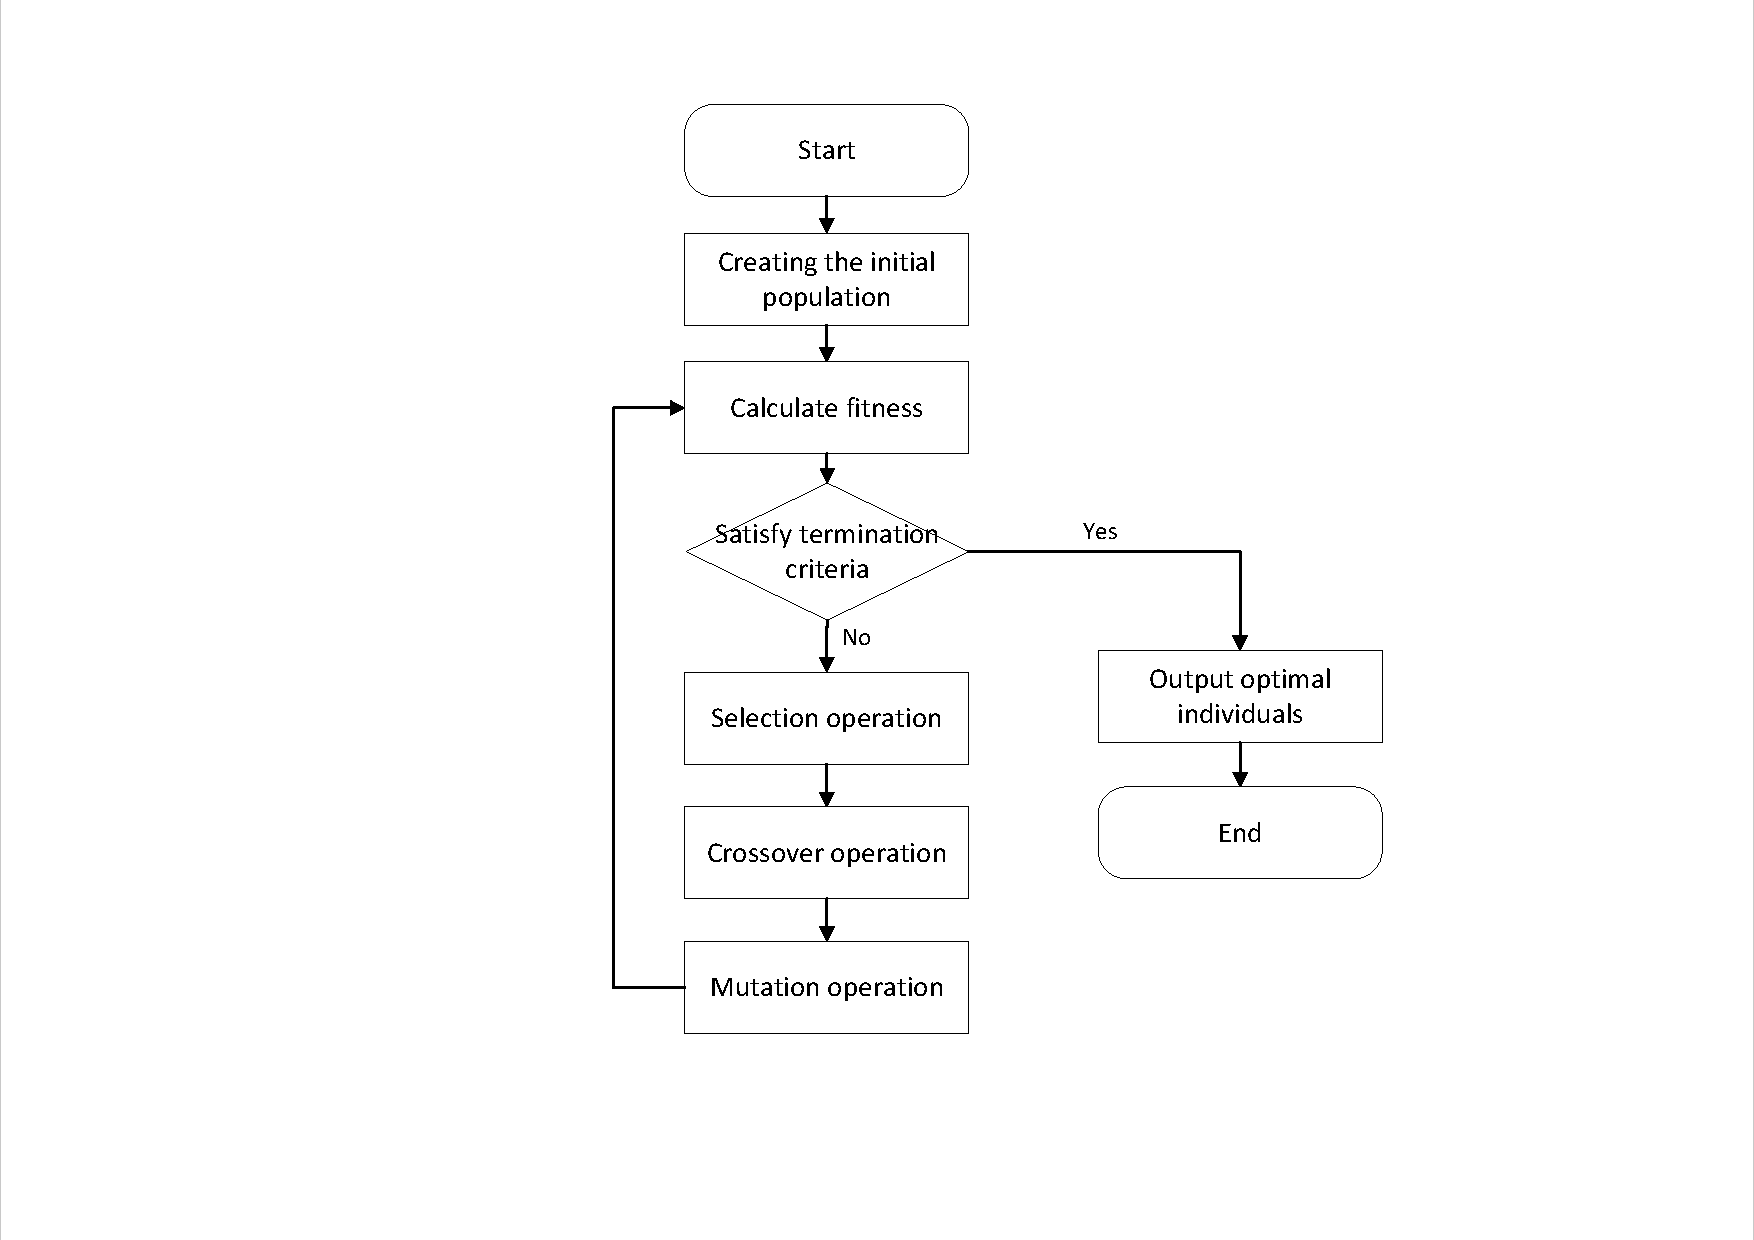
\includegraphics[width=10cm]{C:/Users/31561/Desktop/APMCM LaTeX 模板/figures/GA.pdf}% 图片相对位置
	\caption{Genetic Algorithm Process Diagram} % 图片标题 
	\label{}
\end{figure}

First, a set of design options are randomly generated, each design option is an individual, and all the air-conditioning design options are the initial population.

The objective of the fitness function is to evaluate the advantages and disadvantages of each air conditioning design option, taking into account aspects such as the volume of the air conditioner and the effect of the air conditioner on the temperature of the space. The volume of the air conditioner can be calculated by means of a cylinder.
\begin{equation}
	V = \pi  \cdot radiu{s^2} \cdot h
\end{equation}
Where radius is the radius of the air conditioner and $h$ is the height of the air conditioner.
The effect of air conditioning on space temperature can be modeled by a decay function. Its range of influence is affected by the radius radius of the air conditioner.
\begin{equation}
	{T_{n + 1}} = {T_n} + w(X,Y,Z) \times \left( {{T_{ac\_out}} - {T_n}} \right)
\end{equation}
Where ${T_{n + 1}}$ is the updated temperature field, ${T_n}$  is the current temperature field, and ${T_{ac\_out}}$ is the air outlet temperature of the air conditioner.

After the temperature field is updated, the temperature deviation can be calculated:
\begin{equation}TD= \sum\limits_{X,Y,Z}^{} {\left| {{T_{new}}\left( {X,Y,Z} \right) - {T_{t\arg et}}} \right|} \end{equation}

Where TD denotes temperature deviation.The overall temperature deviation obtained by the above summation is used as the degree of adaptation, where a smaller degree of adaptation indicates a better design.

The selection operation can be performed using a tournament selection algorithm, in which a number of individuals are randomly selected from the population at a time for comparison, and the individual with the highest fitness is selected to go into the next generation. Its simulation formula is:
\begin{equation}
	{X_{selected}} = \arg {\max _{x \in Group}}Fitness(X)
\end{equation}

The crossover operation generates new individuals by selecting two of the screened individuals as parents and exchanging some of the genes in both of them. That is, in two of the designs under screening, some of the design parameters are exchanged to generate a new design. The mutation operation is based on the Gaussian distribution to change some parameters of the individual design in small magnitude immediately.

After several computational iterations, the termination criterion is to reach the target temperature. The best individual that meets the conditions is derived, i.e., the design of the air conditioner. The results obtained above are used as the basic parameters of the air conditioner to study its operation in the room.

The temperature change modeled by this process is based on the heat transfer equation, a partial differential equation of the following form
\begin{equation}
	\rho C\frac{{\partial T}}{{\partial t}} - \nabla  \cdot \left( {k\nabla T} \right) = Q
\end{equation}

where $\rho $ is the density of the material, $C$ is the specific heat capacity of the material, $k$ is the thermal conductivity of the material, and $Q$ is the Joule heat source.

Since the heat source term  is not considered, the above equation can be written as
\begin{equation}
	\frac{{\partial T}}{{\partial t}} = \alpha \left( {\frac{{{\partial ^2}T}}{{\partial {x^2}}} + \frac{{{\partial ^2}T}}{{\partial {y^2}}} + \frac{{{\partial ^2}T}}{{\partial {z^2}}}} \right)
\end{equation}

\begin{equation}
	\alpha  = \frac{k}{{\rho C}}
\end{equation}

\subsubsection{Solution of heat conduction model based on explicit finite difference method}
In the genetic algorithm for iterative solution, so that the volume of air conditioning does not exceed 0.1m³, the selection of the operation to choose three individuals for comparison, the choice of the number of iterations is 50 times. The design scheme is obtained as shown below
\begin{figure}[H]
	\centering
	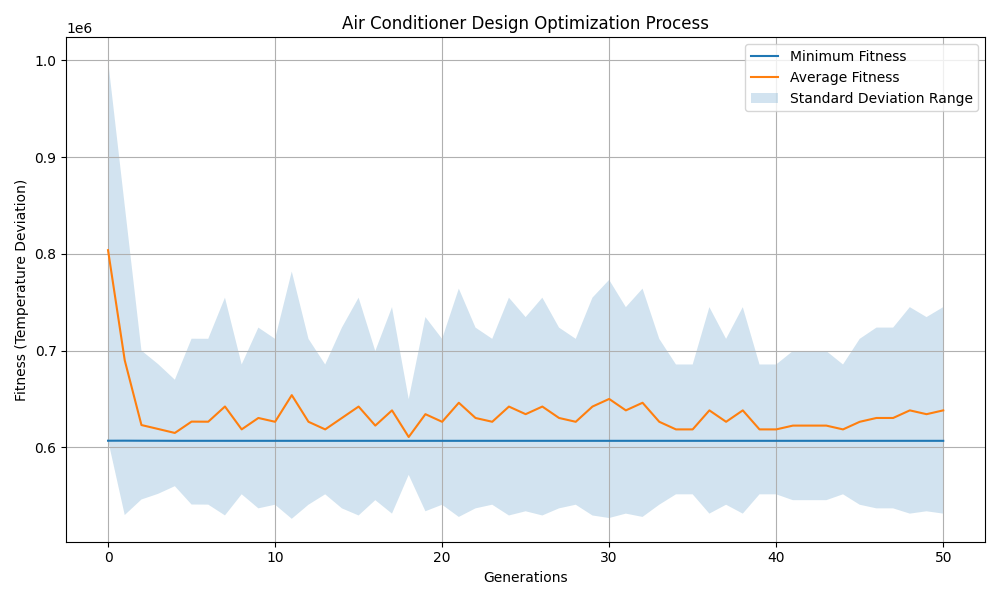
\includegraphics[width=10cm]{q1_ac_design_optimization_ga}% 图片相对位置
	\caption{Plot of results for 50 iterations of the genetic algorithm} % 图片标题 
\end{figure}

Combining the Python results yields an optimal radius for the air conditioner of 0.25 m and a height of 0.5 m. Its design is shown below.
\begin{figure}[H]
	\centering
	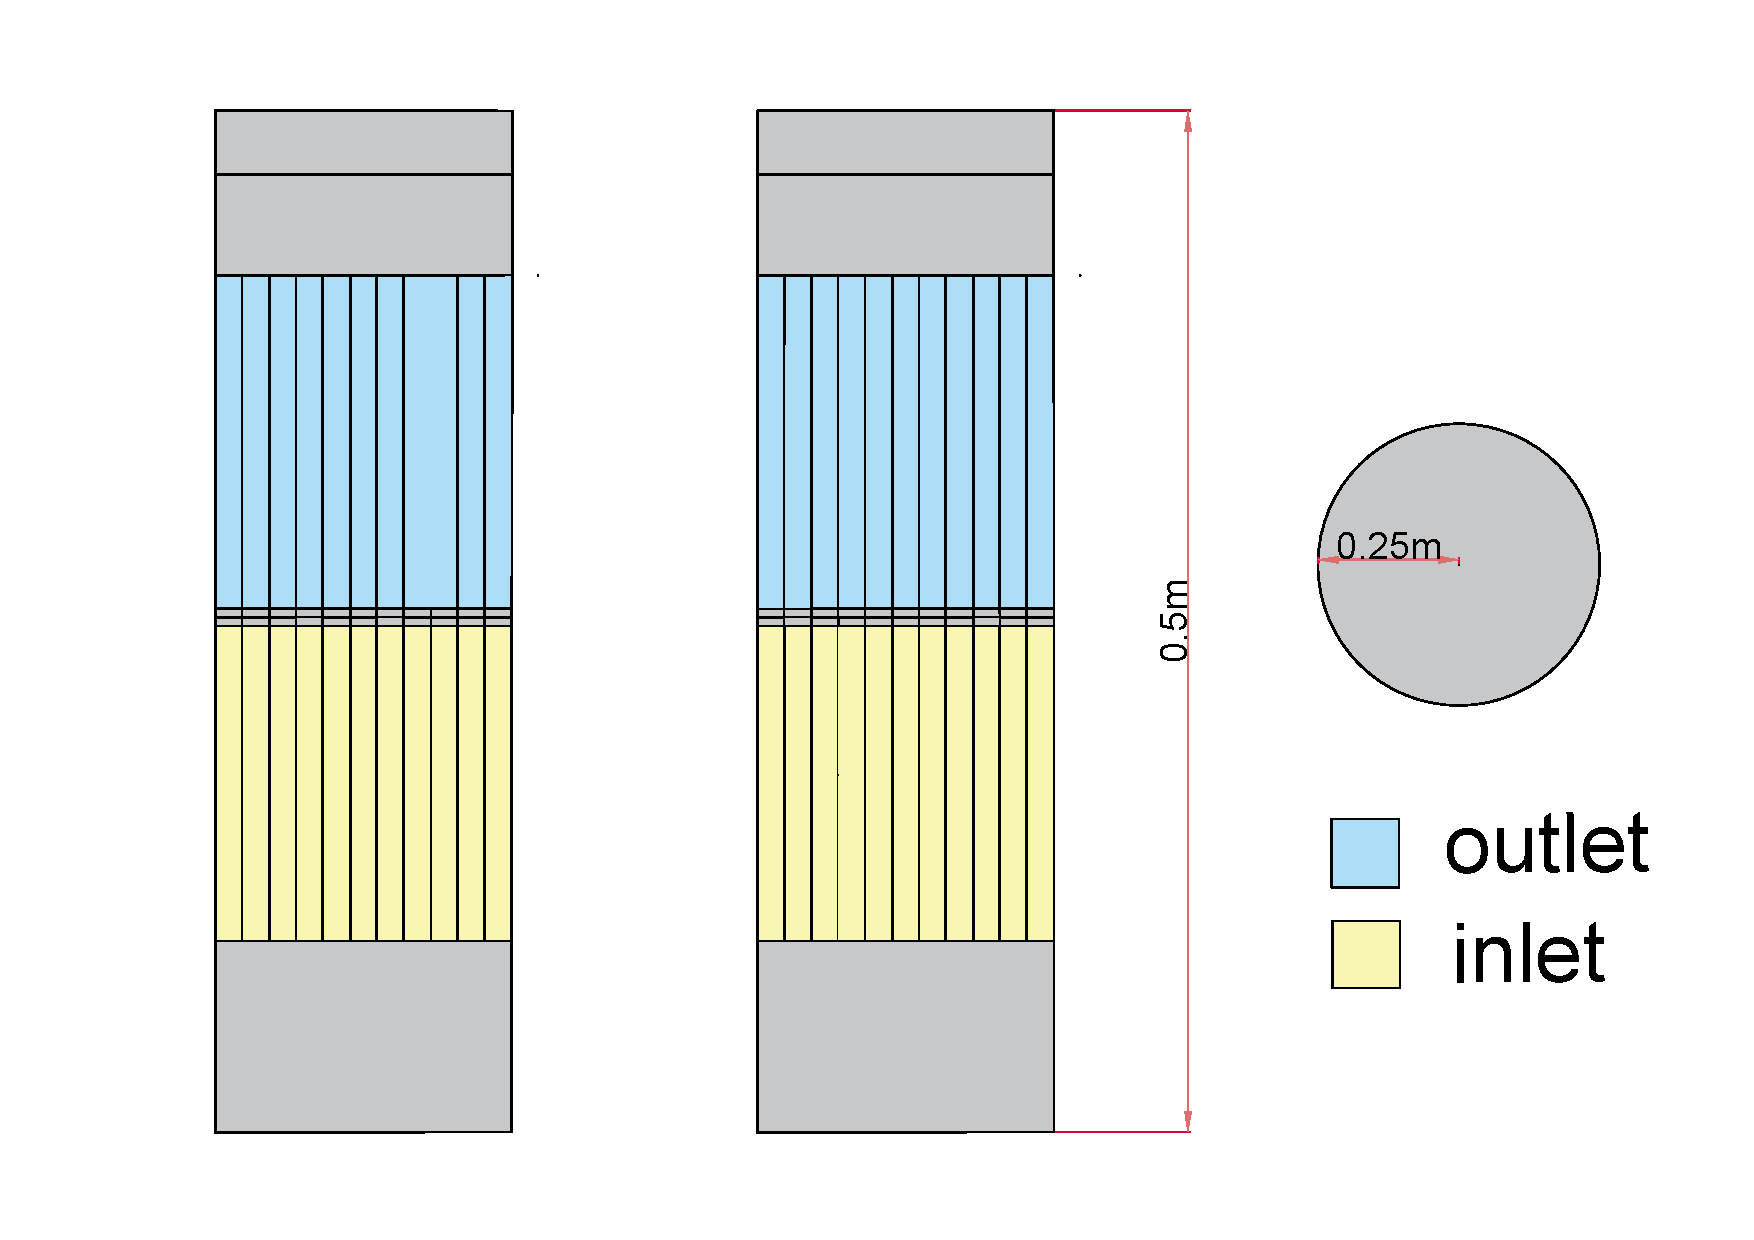
\includegraphics[width=10cm]{kongtiao}% 图片相对位置
	\caption{Optimal Air Conditioner Design} % 图片标题 
\end{figure}

In solving the heat equation for the operation of an air conditioner, time and space can be discretized by the finite difference method.  is the time step and  is the space step, and the space is divided into small grid points at which the temperature is calculated. The time variables are discretized by forward difference and the space vectors are discretized first by forward difference and then by backward difference.

Then the value of the temperature at the grid point  in 3D space at the next time step can be expressed by the following equation
\begin{equation}
	T_{i,j,k}^{n + 1} = T_{i,j,k}^n + \Delta t \cdot \alpha  \cdot {\nabla ^2}C
\end{equation}
Among them.
\begin{equation}
	{\nabla ^2}C = \frac{{T_{i + 1,j,k}^n - 2T_{i,j,k}^n + T_{i - 1,j,k}^n}}{{\Delta {x^2}}} + \frac{{T_{i,j + 1,k}^n - 2T_{i,j,k}^n + T_{i,j - 1,k}^n}}{{\Delta {y^2}}} + \frac{{T_{i,j,k + 1}^n - 2T_{i,j,k}^n + T_{i,j,k - 1}^n}}{{\Delta {z^2}}}
\end{equation}

where $T_{i,j,k}^{n + 1}$ is the next time step at $n + 1$ ,
$T_{i,j,k}^n$ is the current time step at $n$ , and ${\nabla ^2}C$ is the Laplace operator.

In summer, the boundary temperature was set to 35°C and the air conditioning temperature to 24°C. After the air conditioner works for 30s, 300s and 600s, the indoor temperature distribution is shown in the figure below.
\begin{figure}[H]
	\centering    
	\subfigure[]{				% 图片1([]内为子图标题)
		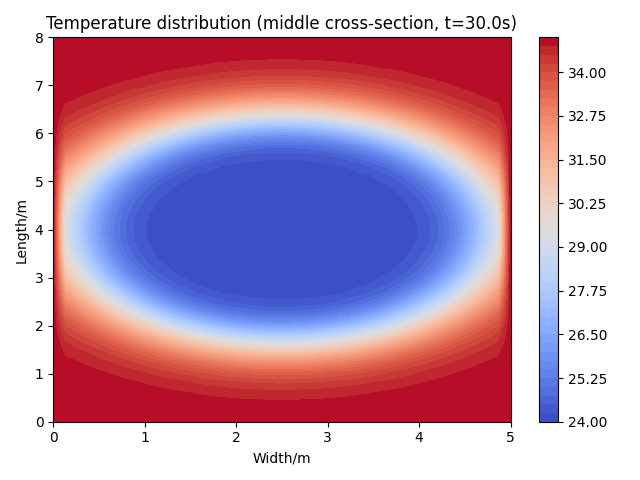
\includegraphics[width=0.3\textwidth]{q1_30.0s_diff_summer}}% 子图1的相对位置
	\subfigure[]{				% 图片2
		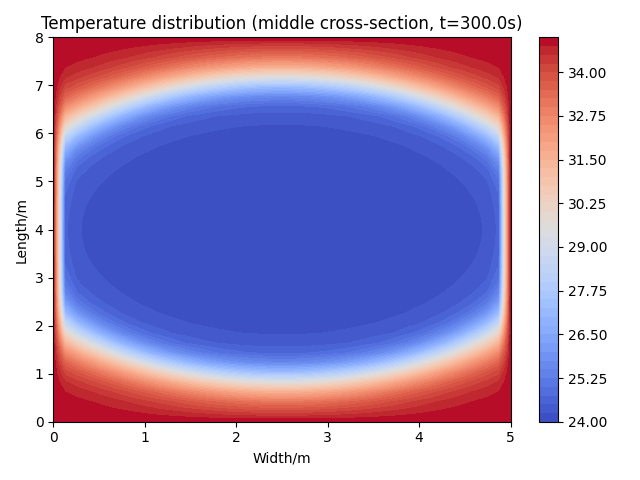
\includegraphics[width=0.3\textwidth]{q1_300.0s_diff_summer}}% 子图2的相对位置
	\subfigure[]{				% 图片2
		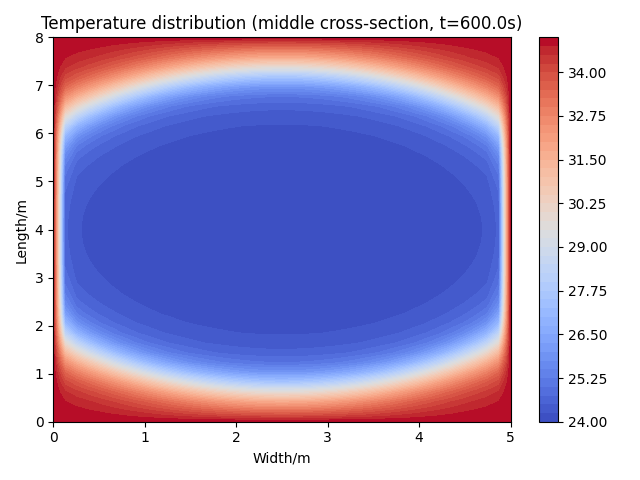
\includegraphics[width=0.3\textwidth]{q1_600.0s_diff_summer}}% 子图3的相对位置
	\caption{Temperature distribution in a two-dimensional plane after 30, 300 and 600 seconds}		% 总图标题
\end{figure}
\begin{figure}[H]
	\centering    
	\subfigure[]{				% 图片1([]内为子图标题)
		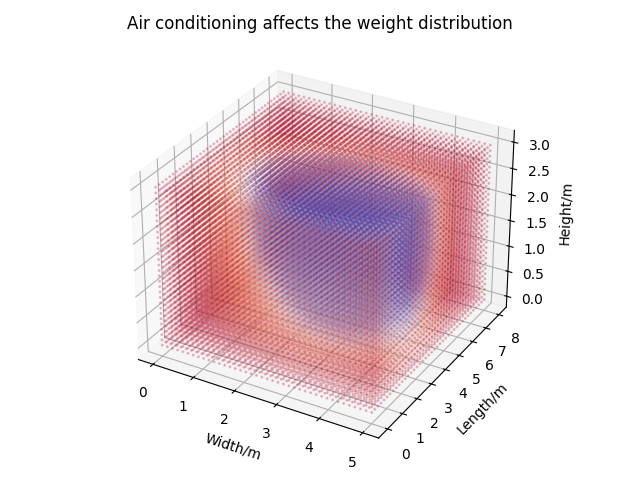
\includegraphics[width=0.3\textwidth]{q1_30.0s_scatter_summer}}% 子图1的相对位置
	\subfigure[]{				% 图片2
		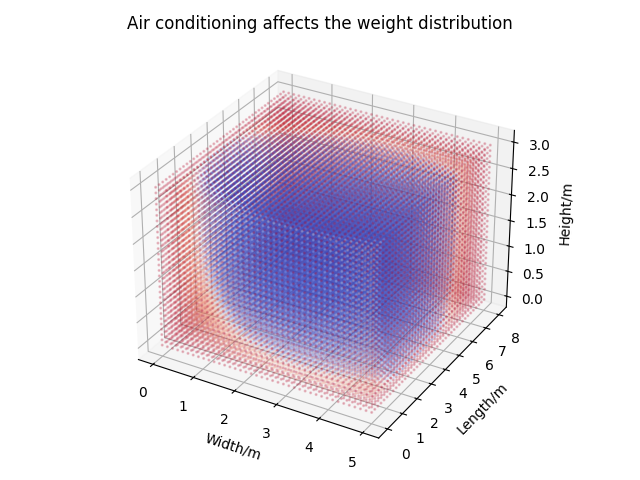
\includegraphics[width=0.3\textwidth]{q1_300.0s_scatter_summer}}% 子图2的相对位置
	\subfigure[]{				% 图片2
		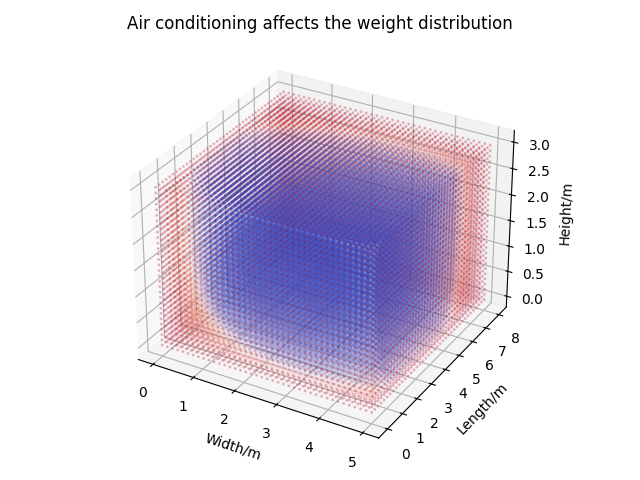
\includegraphics[width=0.3\textwidth]{q1_600.0s_scatter_summer}}% 子图3的相对位置
	\caption{Temperature distribution in a three-dimensional plane after 30, 300 and 600 seconds.}		% 总图标题
\end{figure}

With time, the temperature of the indoor two-dimensional thermal field decreases gradually from the location of the air conditioner in all directions, and the temperature of the three-dimensional scattering points decreases gradually from the location of the air conditioner in all directions within the space. The average indoor temperature over time is plotted below.
\begin{figure}[H]
	\centering
	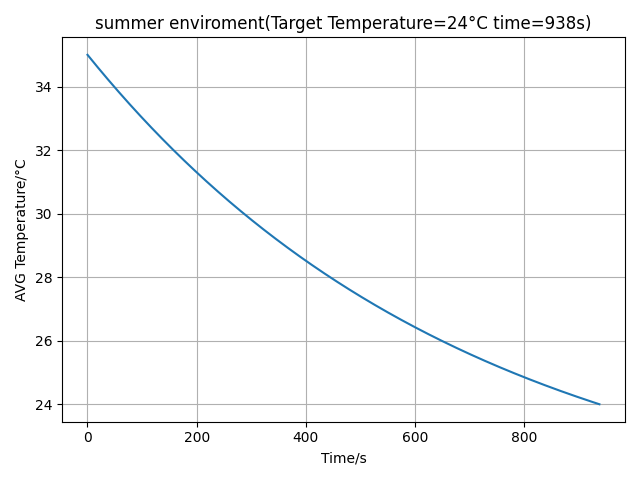
\includegraphics[width=8cm]{q1_avg_temperature_summer}% 图片相对位置
	\caption{Temperature versus time graph} % 图片标题 
\end{figure}

According to the Python calculations, it can be seen that when the time is 938s, the average indoor temperature reaches 24°C, which is in line with the expected indoor temperature.

In summer, the boundary temperature was set to 5°C and the air conditioning temperature was 24°C. After the air conditioner works for 30s, 300s and 600s, the indoor temperature distribution is shown below.

\begin{figure}[H]
	\centering    
	\subfigure[]{				% 图片1([]内为子图标题)
		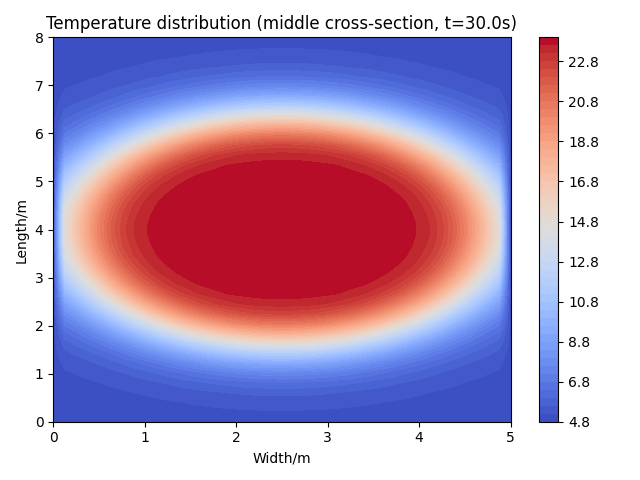
\includegraphics[width=0.3\textwidth]{q1_30.0s_diff_winter}}% 子图1的相对位置
	\subfigure[]{				% 图片2
		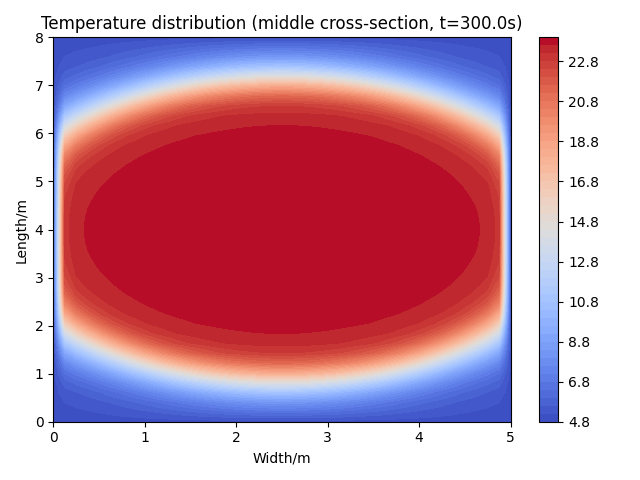
\includegraphics[width=0.3\textwidth]{q1_300.0s_diff_winter}}% 子图2的相对位置
	\subfigure[]{				% 图片2
		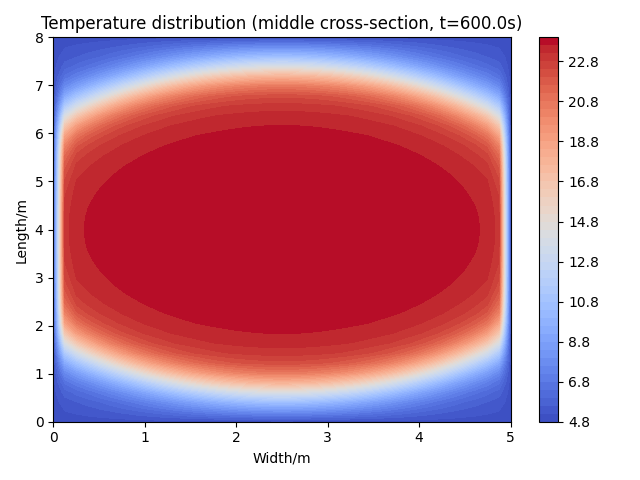
\includegraphics[width=0.3\textwidth]{q1_600.0s_diff_winter}}% 子图3的相对位置
	\caption{Temperature distribution in a two-dimensional plane after 30, 300 and 600 seconds}		% 总图标题
\end{figure}
\begin{figure}[H]
	\centering    
	\subfigure[]{				% 图片1([]内为子图标题)
		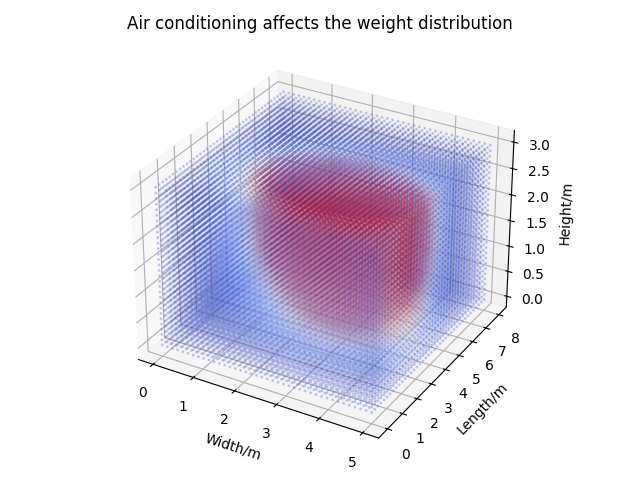
\includegraphics[width=0.3\textwidth]{q1_30.0s_scatter_winter}}% 子图1的相对位置
	\subfigure[]{				% 图片2
		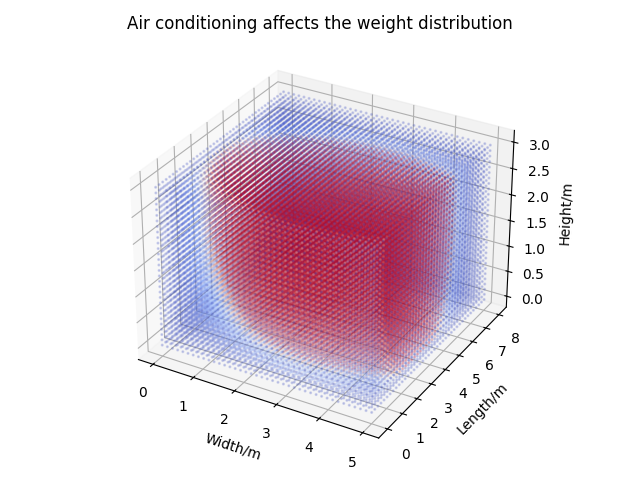
\includegraphics[width=0.3\textwidth]{q1_300.0s_scatter_winter}}% 子图2的相对位置
	\subfigure[]{				% 图片2
		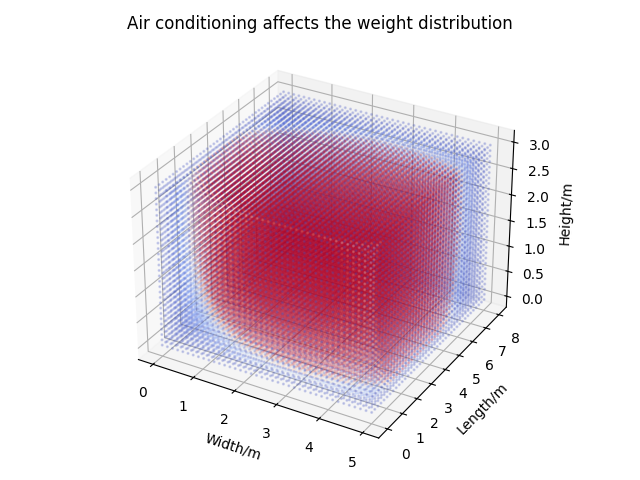
\includegraphics[width=0.3\textwidth]{q1_600.0s_scatter_winter}}% 子图3的相对位置
	\caption{Temperature distribution in a three-dimensional plane after 30, 300 and 600 seconds}		% 总图标题
\end{figure}
With time, the temperature of the indoor two-dimensional thermal field gradually increases from the location of the air conditioner in all directions, and the temperature of the three-dimensional scattering points gradually increases from the location of the air conditioner in all directions within the space. The average indoor temperature over time is plotted below.

\begin{figure}[H]
	\centering
	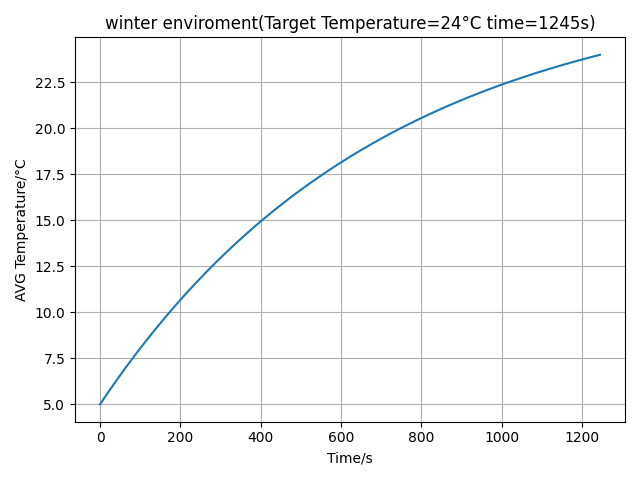
\includegraphics[width=10cm]{q1_avg_temperature_winter}% 图片相对位置
	\caption{Temperature versus time graph} % 图片标题 
\end{figure}
According to the Python calculations, it can be seen that when the time is 1245s, the average indoor temperature reaches 24°C, which is in line with the expected indoor temperature.

In addition, the ANSYS FLUENT \cite{zhu2002concentration}simulation was used to simulate the temperature change in the room after 5 minutes and 10 minutes in summer, and the following figure shows the top-view thermal map at the height of the air conditioning outlet, and the blank space is the position of the air conditioning placement.


\begin{figure}[H]
	\centering
	\begin{minipage}{0.5\textwidth}
		\centering
		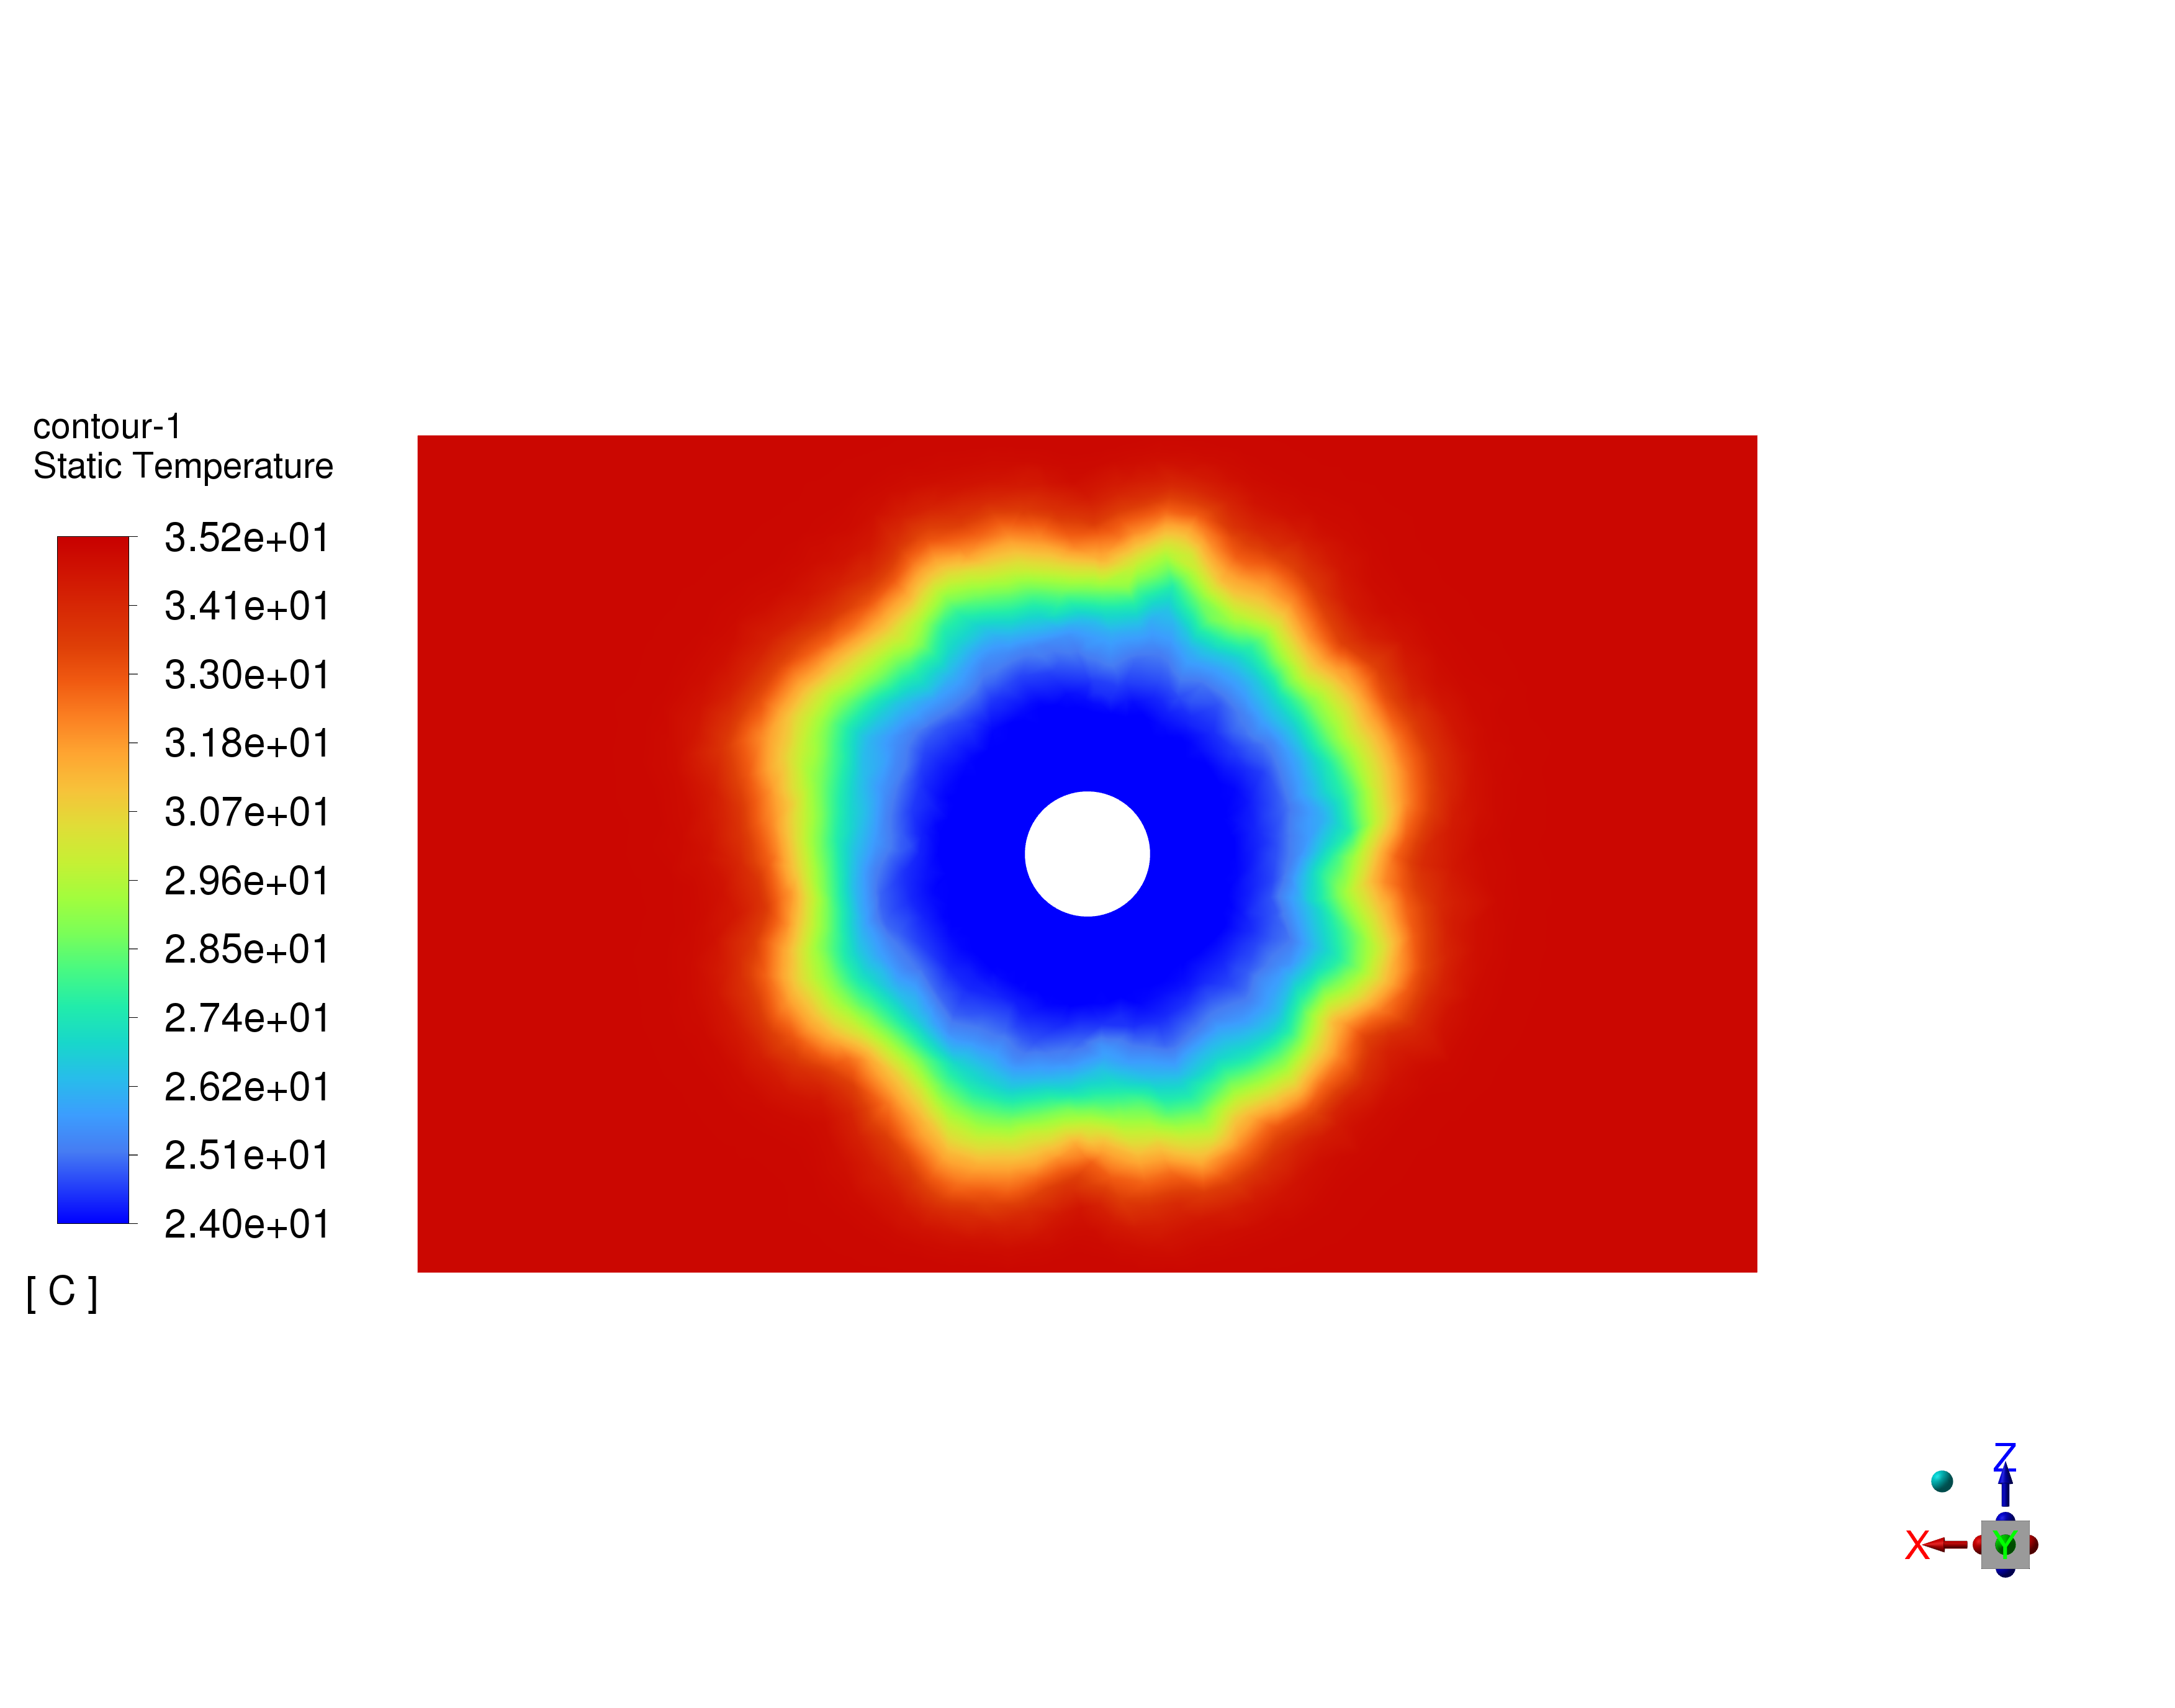
\includegraphics[width=\textwidth]{kongtiao1xywdc}
		\caption{after 5 minutes}
	\end{minipage}%
	\begin{minipage}{0.5\textwidth}
		\centering
		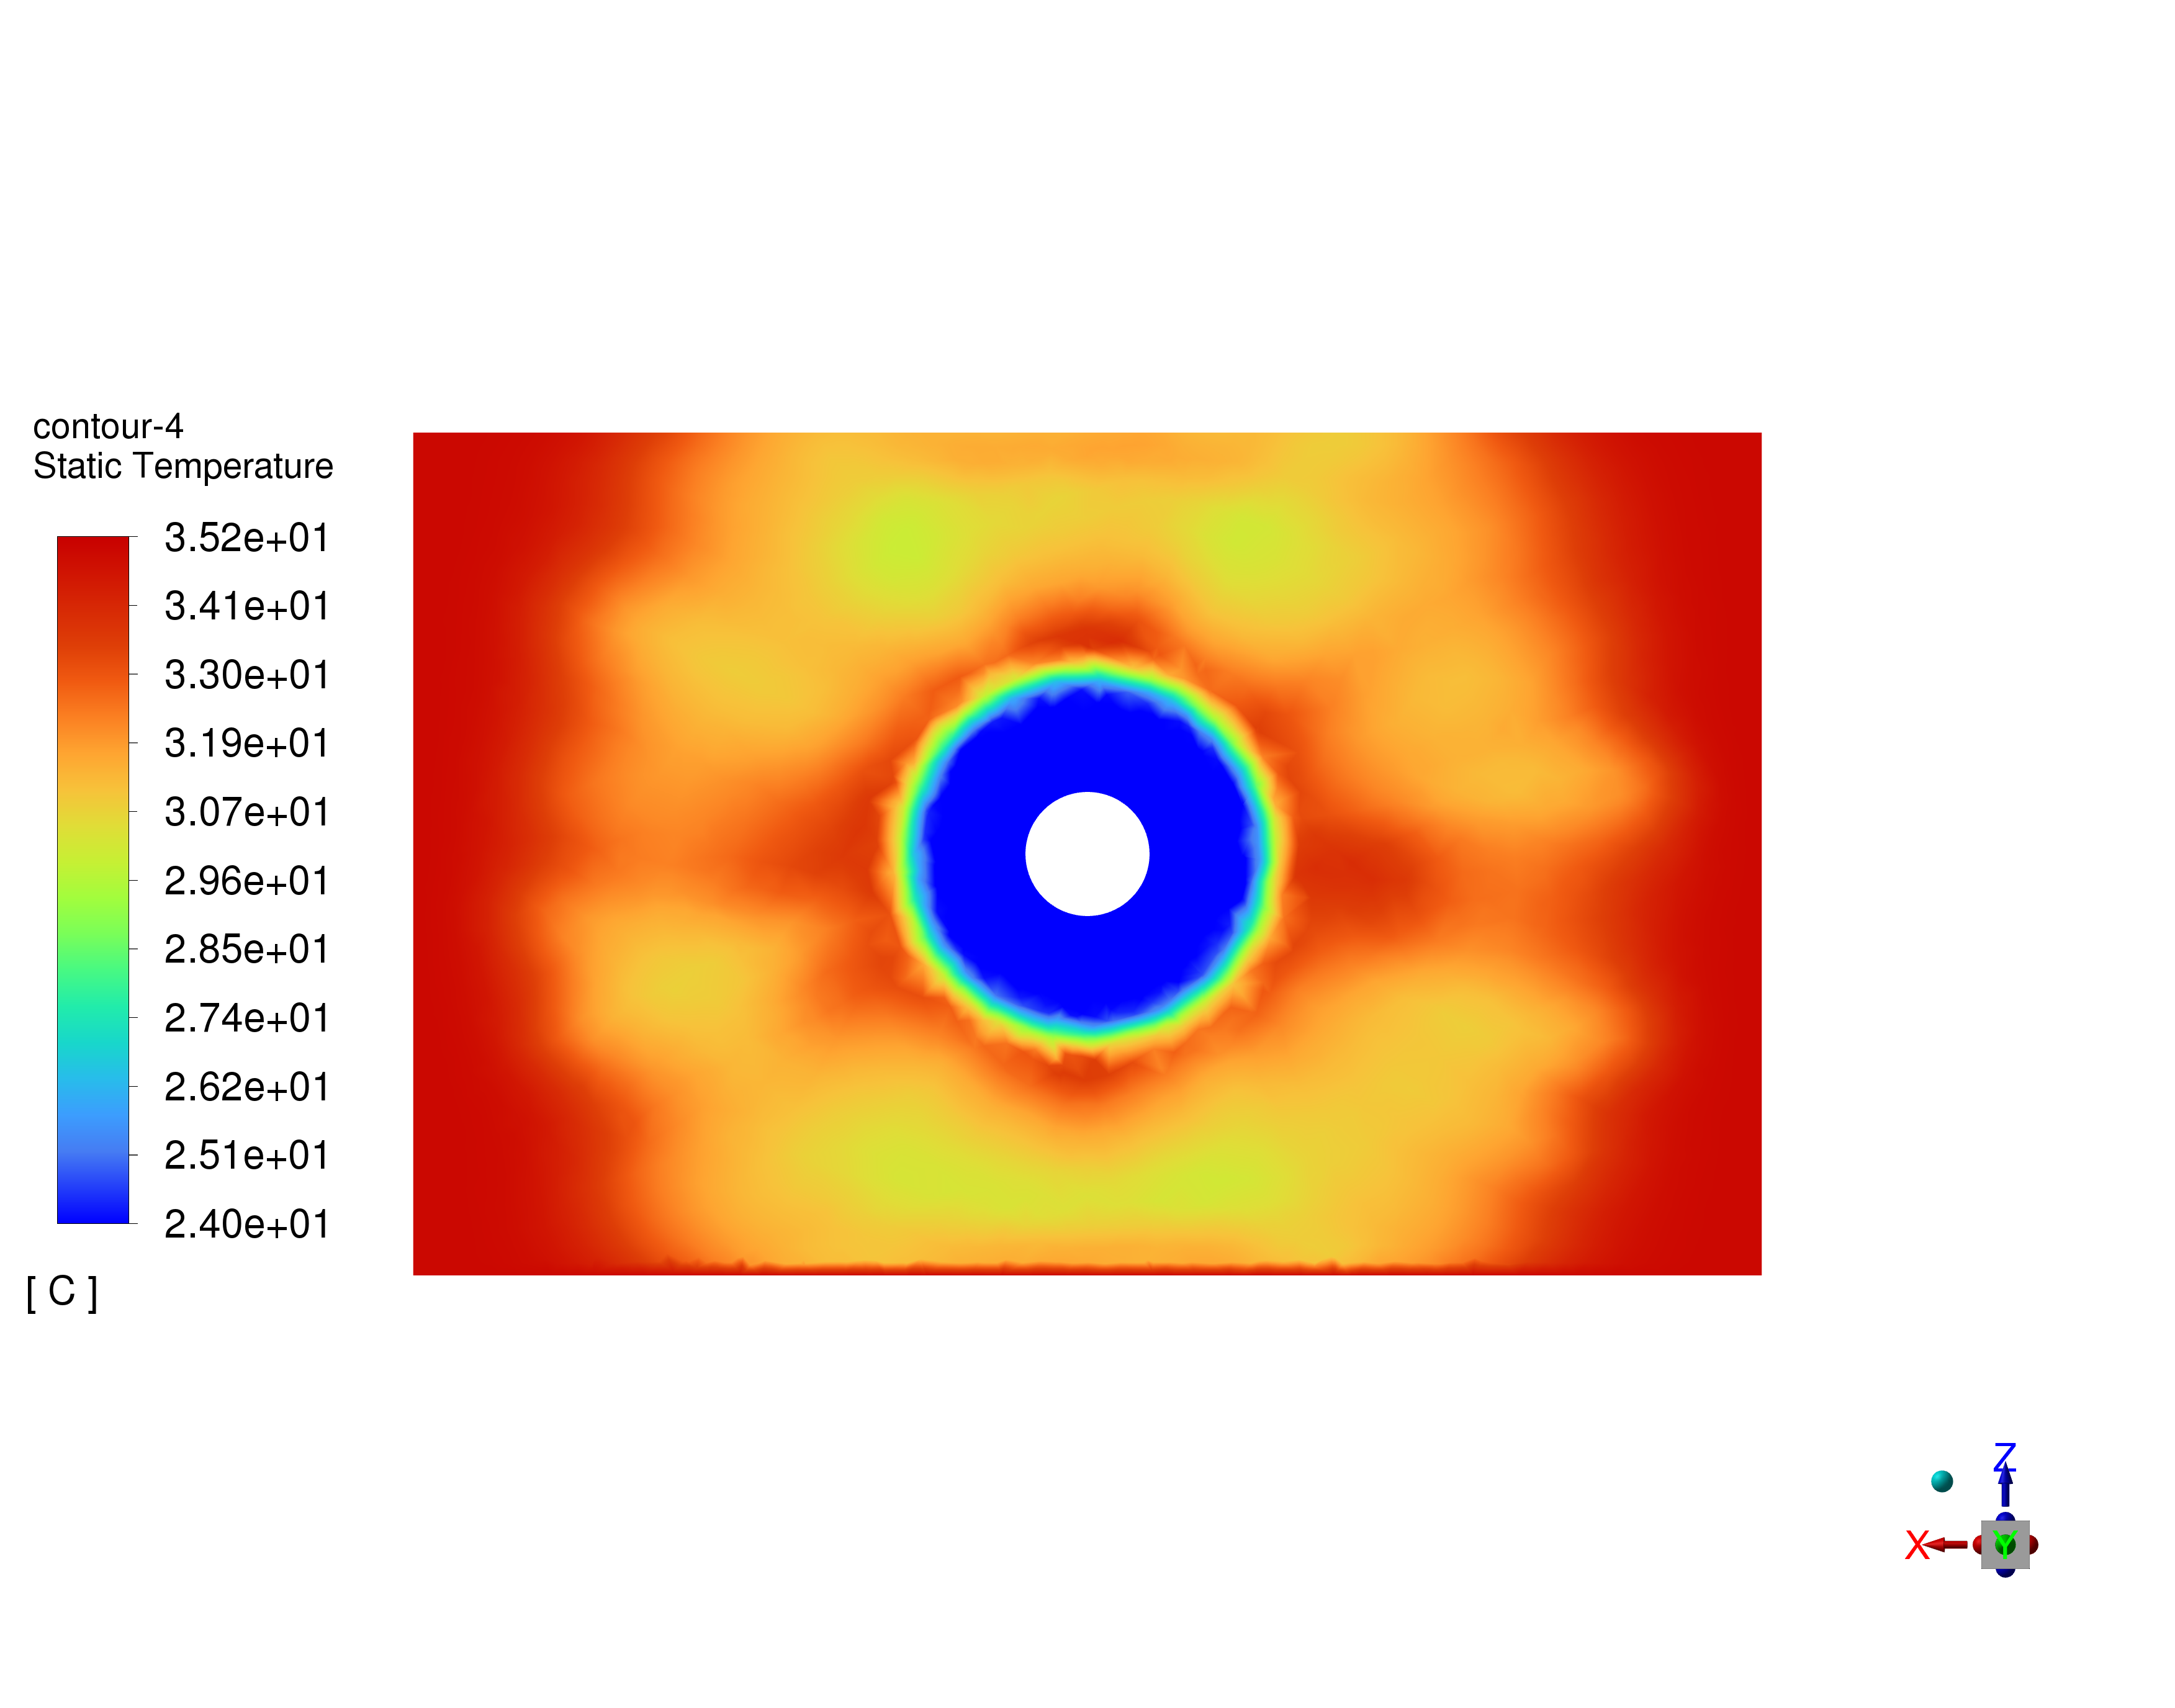
\includegraphics[width=\textwidth]{kong90_xz_wdcplan7}
		\caption{after 10 minutes}
	\end{minipage}
\end{figure}


In winter, the change in room temperature after 5 minutes and 10 minutes are shown below.

\begin{figure}[H]
	\centering
	\begin{minipage}{0.5\textwidth}
		\centering
		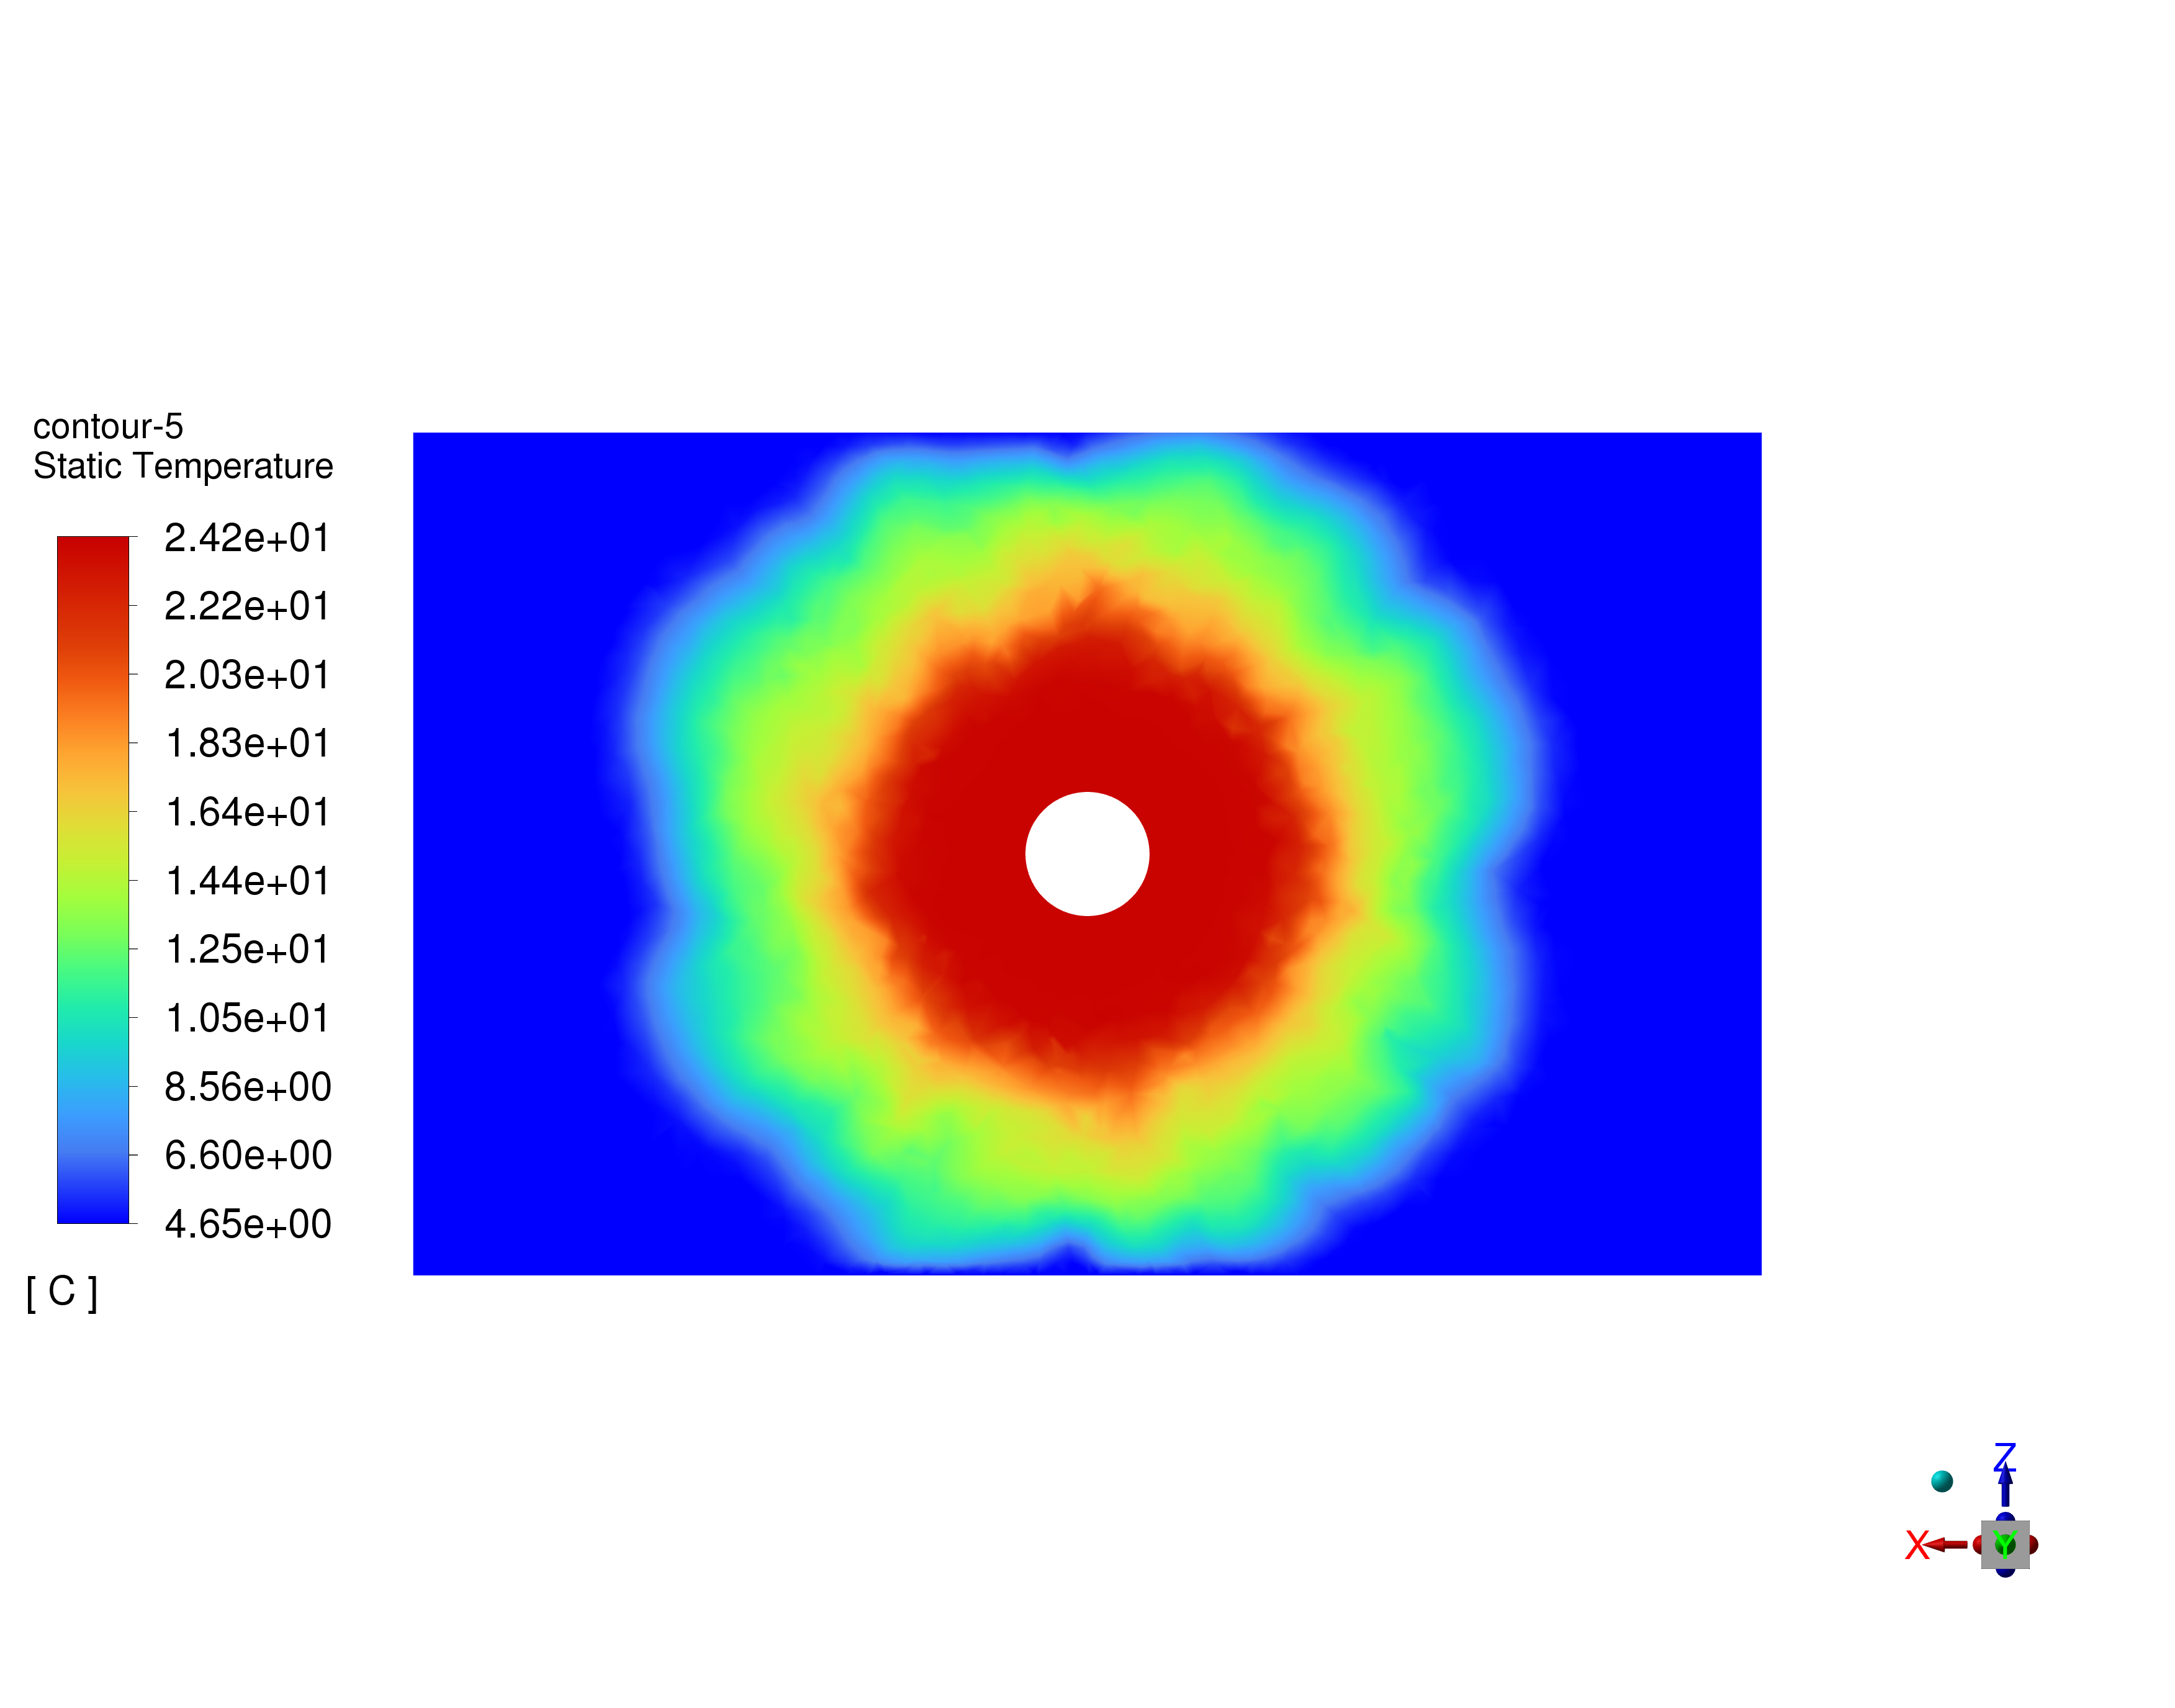
\includegraphics[width=\textwidth]{kong45tiao_xz_wdcplan7}
		\caption{after 5 minutes}
	\end{minipage}%
	\begin{minipage}{0.5\textwidth}
		\centering
		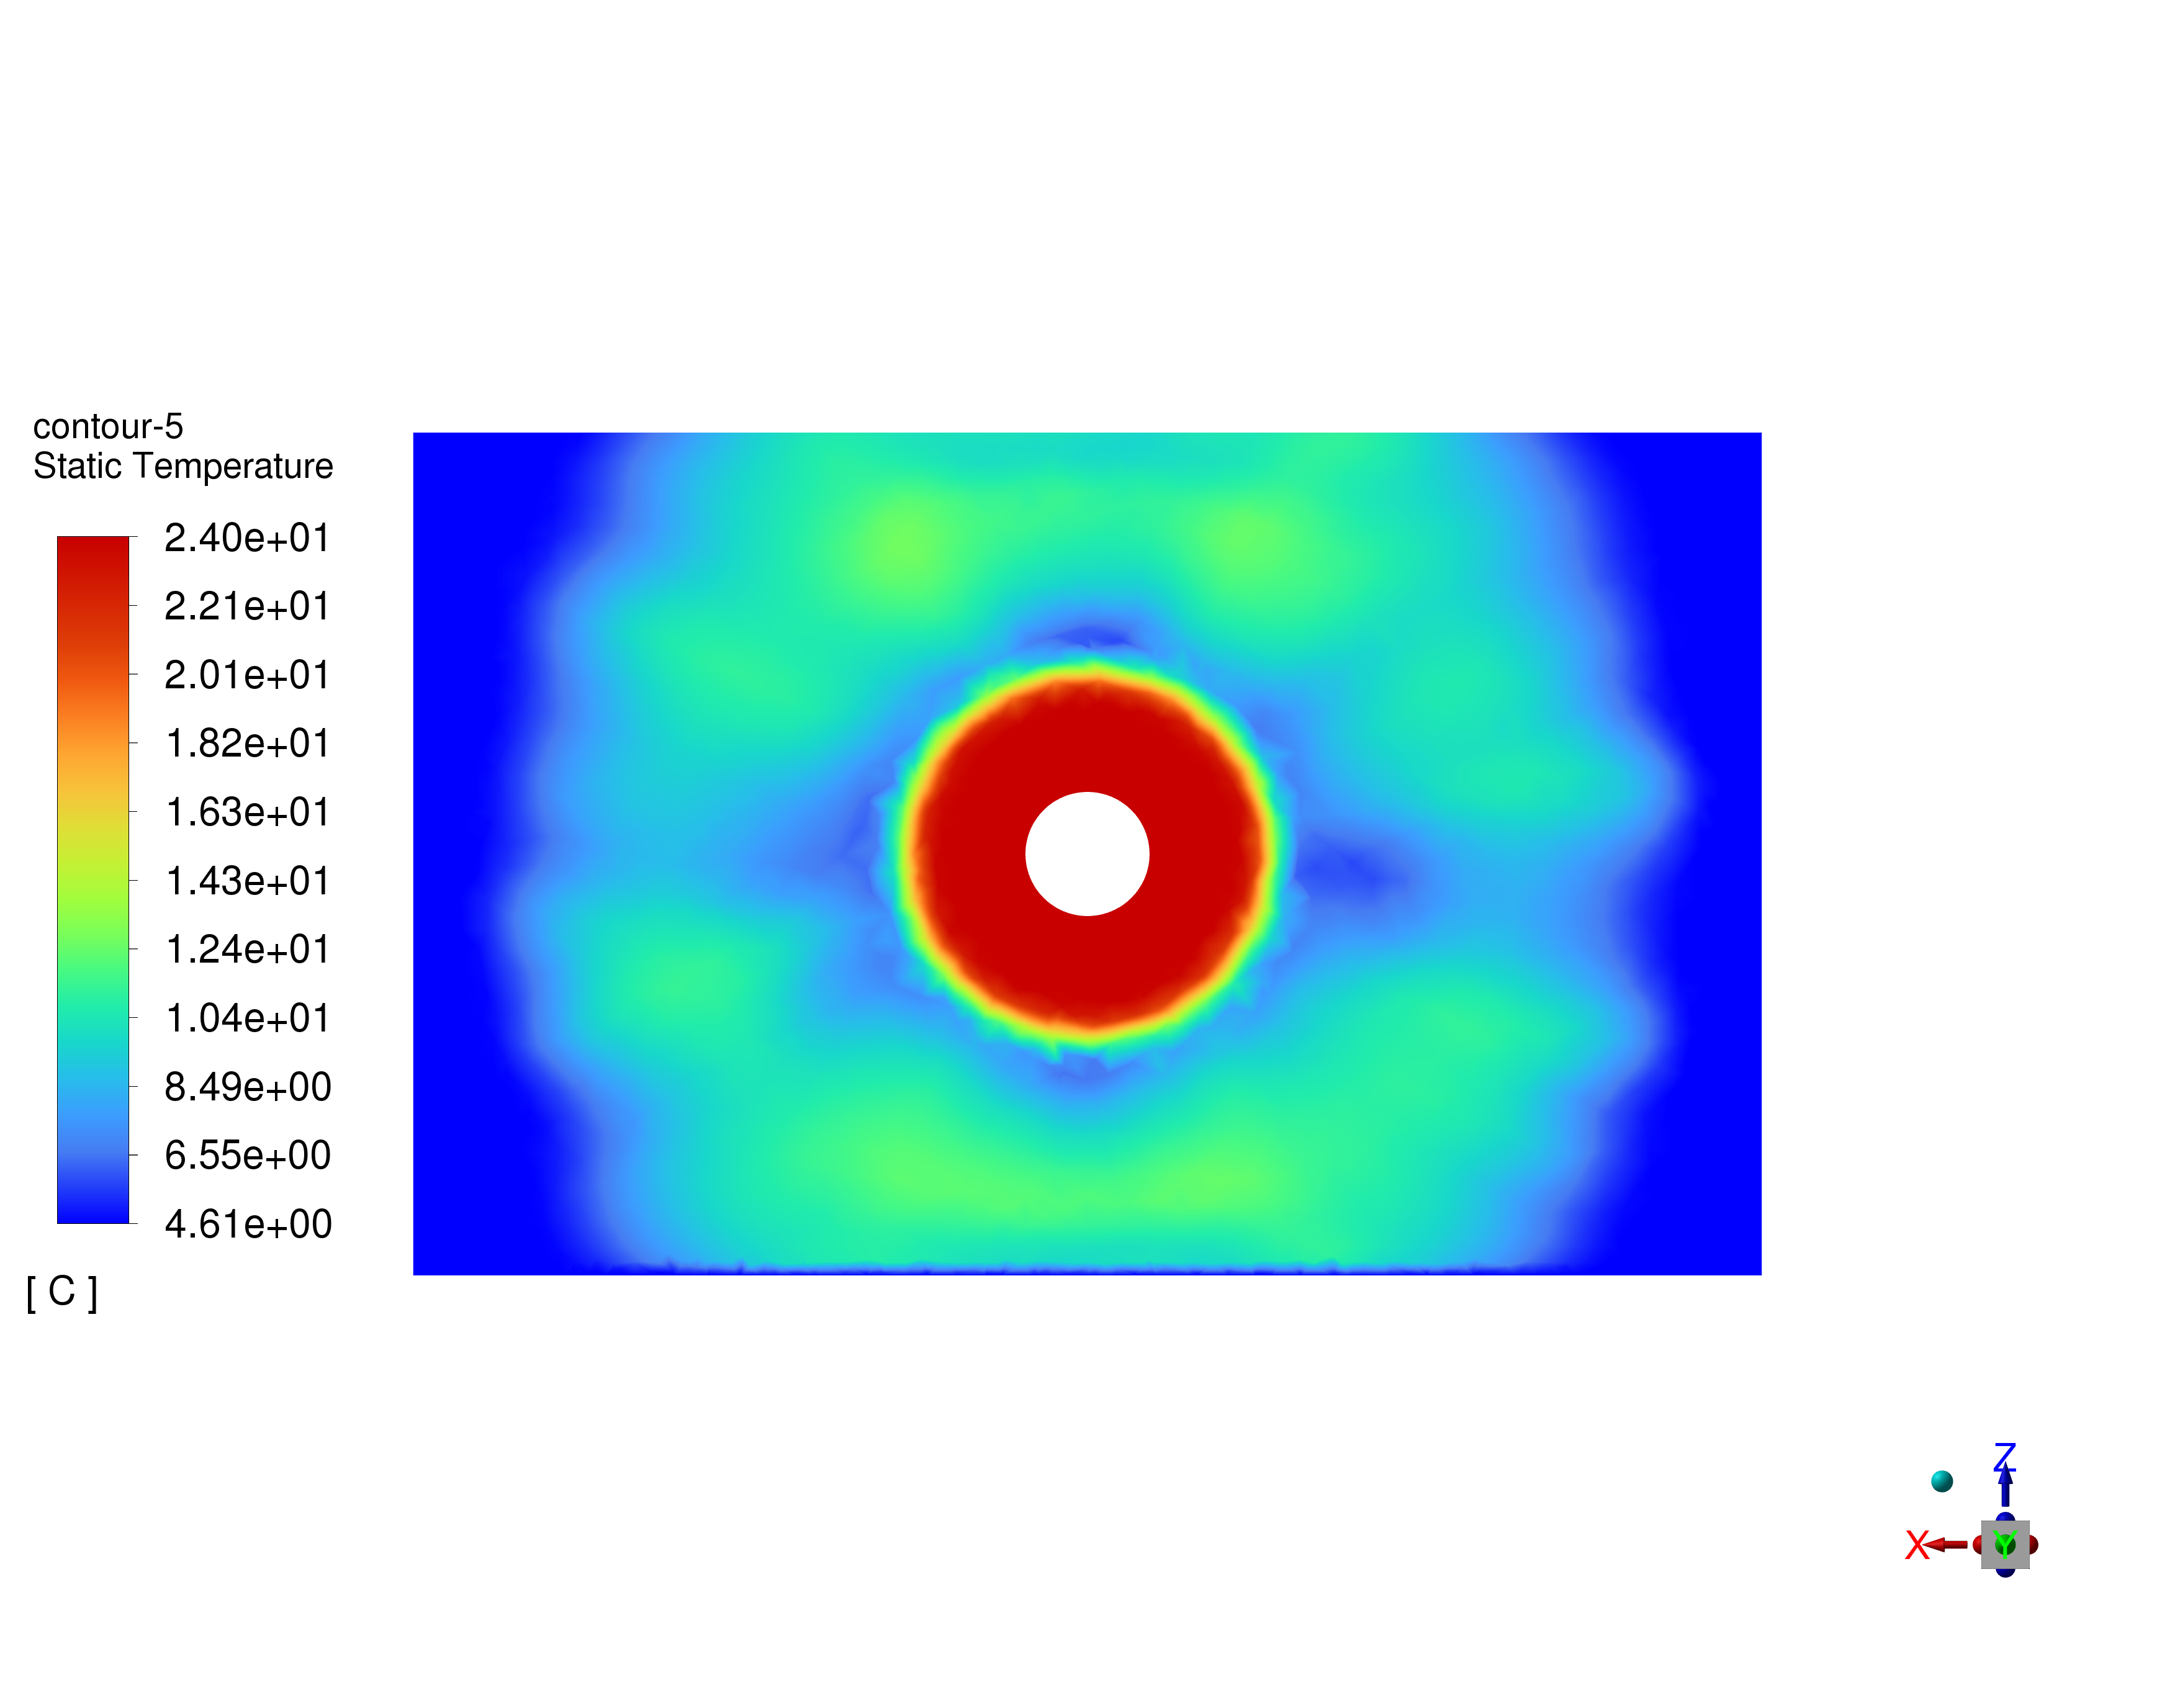
\includegraphics[width=\textwidth]{kong90tiao_xz_wdcplan7}
		\caption{after 10 minutes}
	\end{minipage}
\end{figure}


From the analysis of the results of ANSYS simulation of the indoor temperature field changes, it can be seen that in a certain time, the indoor thermal field changes in line with the Python simulation of the expected two-dimensional thermal field and the plotted temperature change over time graph, which is consistent with the expected results
\begin{figure}[H]
	\centering
	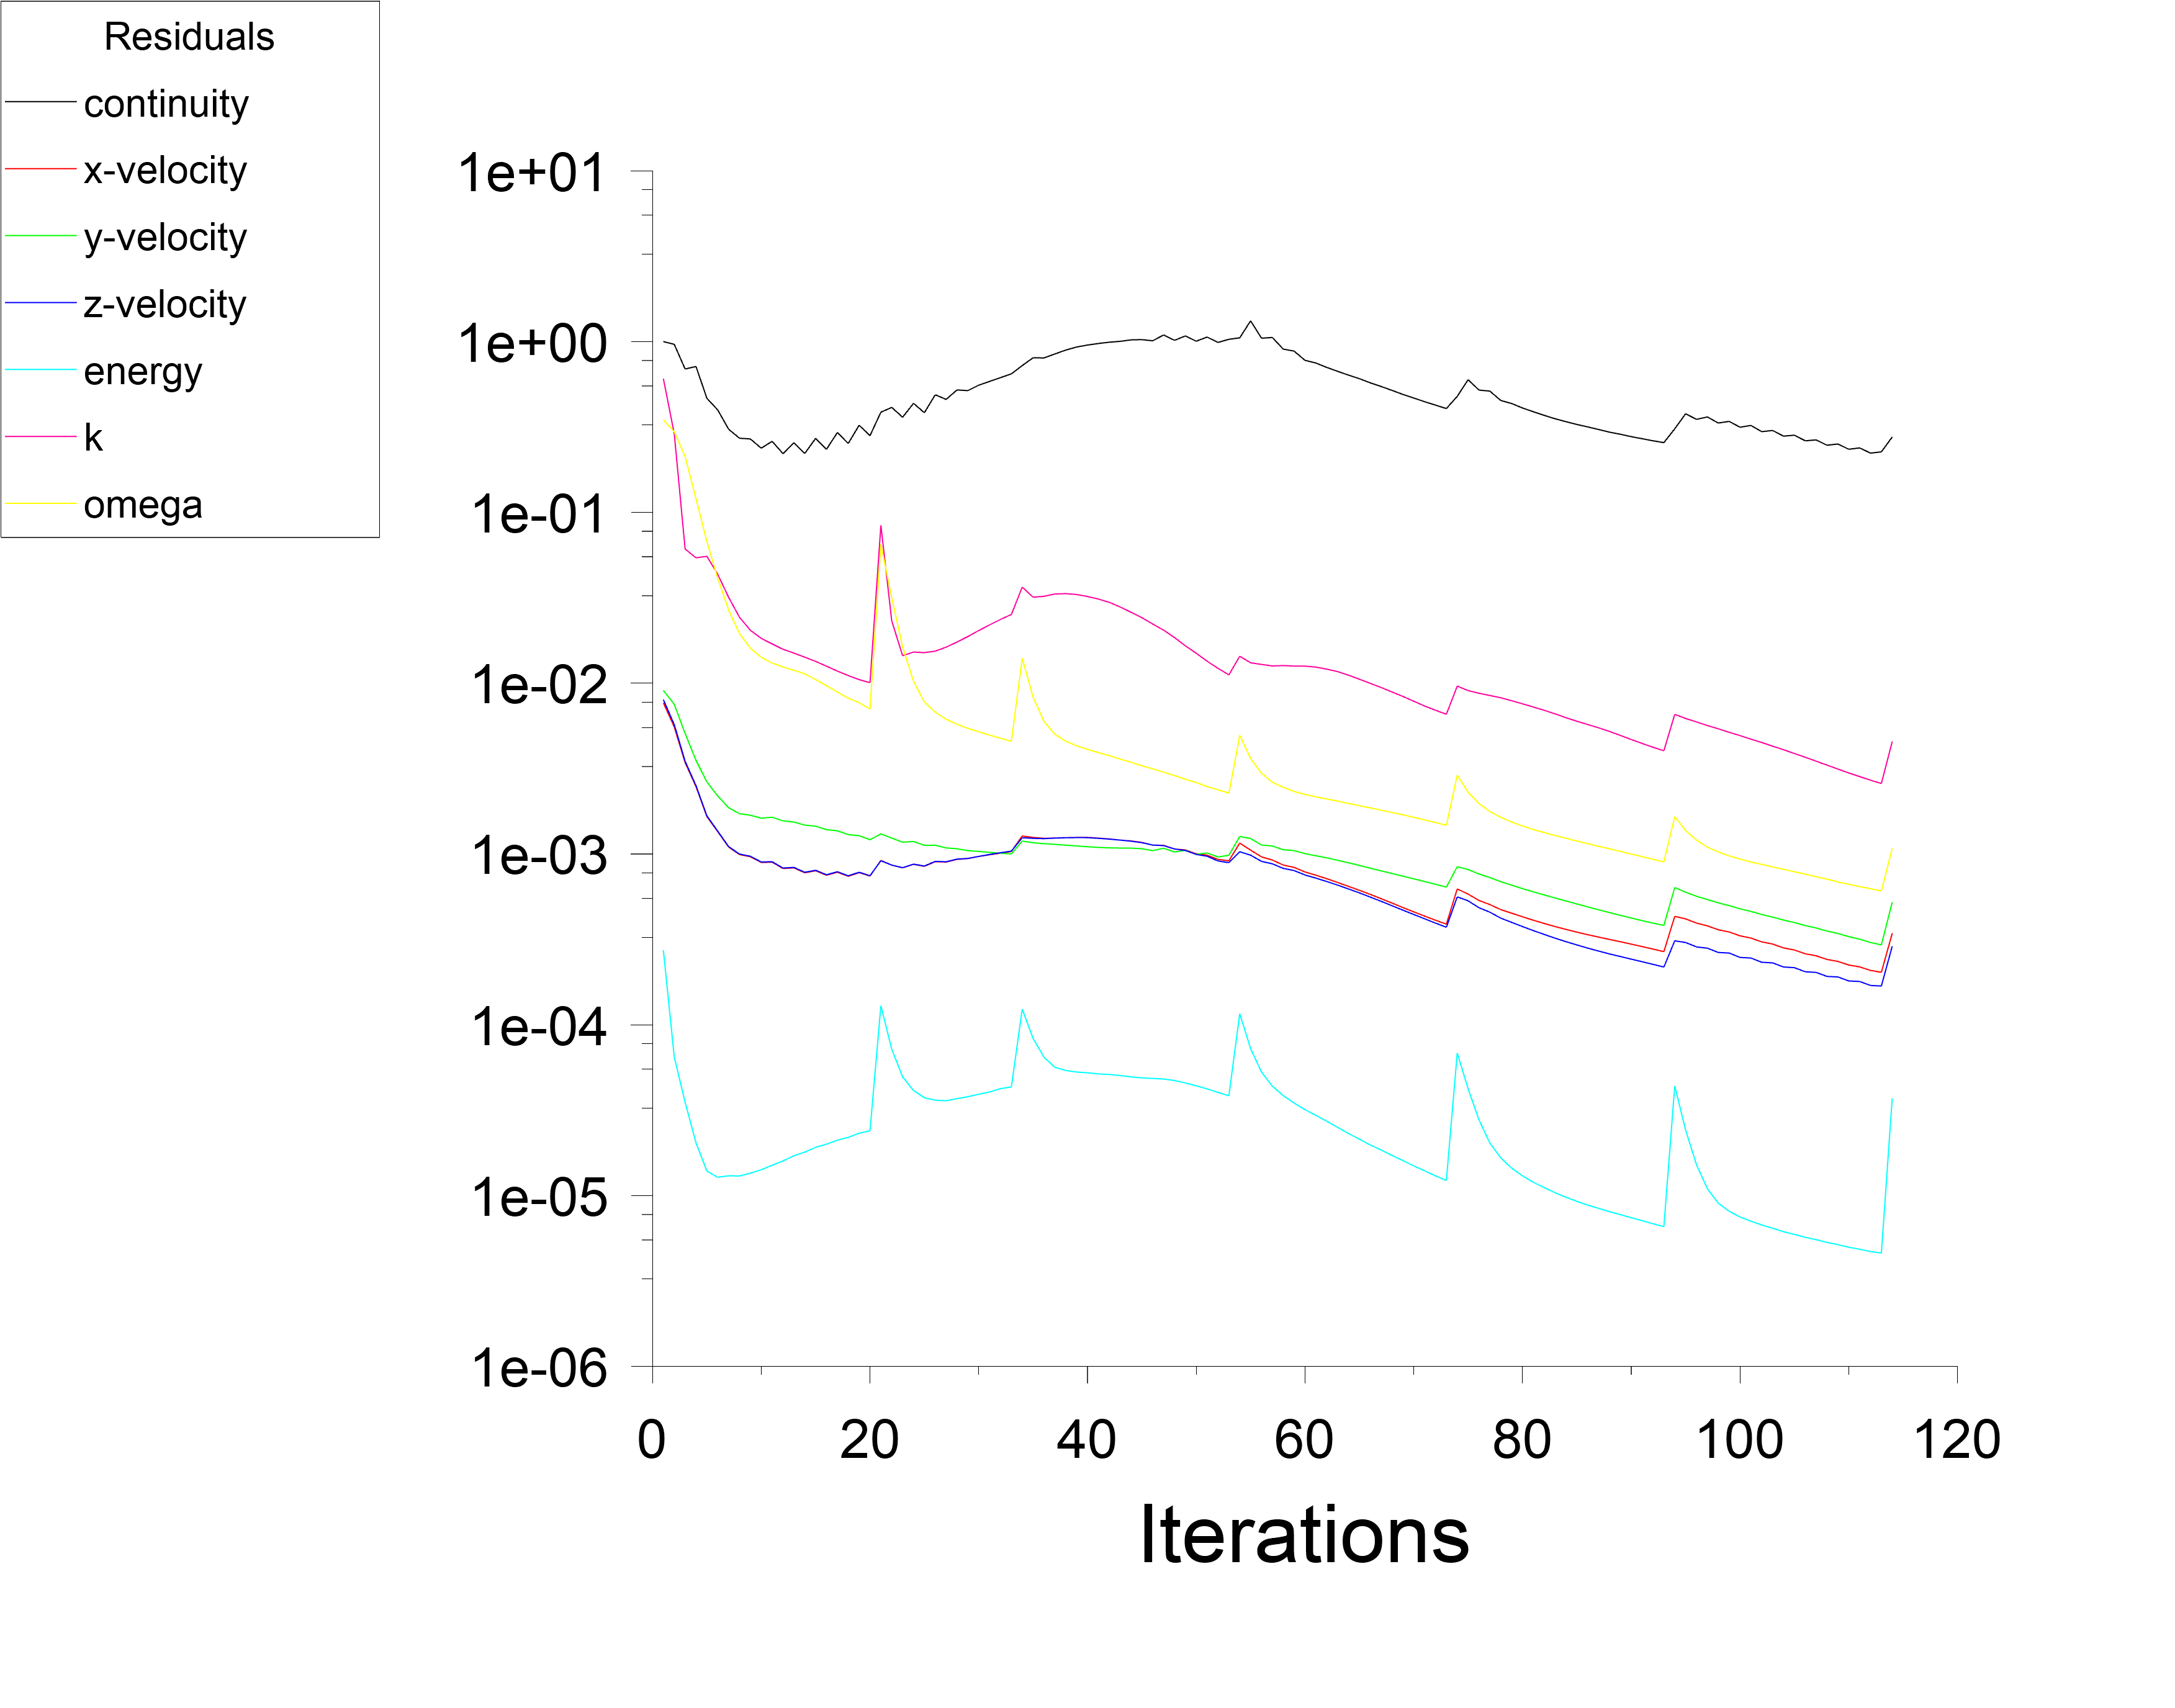
\includegraphics[width=10cm]{kongtiao2x_y_h_sdc1zexiantu}% 图片相对位置
	\caption{residual curve graph} % 图片标题 
\end{figure}
According to the residual table of ANSYS, it can be seen that as the number of iterations increases, the residuals of all physical quantities are decreasing, and the numerical solution is gradually converging to a stable solution, indicating that the solution is good. 

The combined Python and Computational Fluid Dynamics (CFD) software ANSYS FLUENT simulation results show that the exterior design and related parameters of the air conditioner are in line with the expected situation.


\subsubsection{Advantages and Disadvantages of Explicit Finite Difference Method Based Heat Transfer Modeling}
\begin{description}
	\item[Strength:]1. The genetic algorithm used has global search capability to avoid falling into the trap of local optimal solution.
	2. shows that the update of each grid point of the finite difference method is independent and suitable for parallel computation.
	\item[Weakness:]  Genetic algorithms are dependent on the selection of the initial population and the potential capacity of parallel mechanisms is underutilized.
\end{description}
\subsection{Concentration-diffusion modeling and solution based on Fick's second law}
Genetic algorithm to find the optimal air purifier shape and size and Fick's second law to explore the process of indoor pollutant concentration.
\subsubsection{Preparation of a concentration-diffusion model based on Fick's second law}
Also based on the Euclidean distance formula, the distance from any point in the space $\left( {X,Y,Z} \right)$ to the air humidifier $\left( {{x_0},{y_0},{z_0}} \right)$ can be calculated, and substituted into the Gaussian function to calculate the weights of each grid node in the space to simulate the ability of the purifier to reduce the concentration of pollutants at different distances.

According to the relevant literature\cite{sadrizadeh2022indoor} and market research statistics analysis, it is known that the shape of the air purifier is cylindrical as the optimal shape.
\subsubsection{ Modeling of concentration diffusion based on Fick's second law}
The optimal air purifier shape and size can be derived based on genetic algorithm. An initial set of design options is first randomly generated, and all possible purifier design options are the initial population. Each individual consists of several design parameters such as diameter, height, number of filter layers, number of air inlets, and number of air outlets.

\begin{equation}
P = \left\{ {{X_1},{X_2},...,{X_n}} \right\}a
\end{equation}

where each Xi is a vector of individual design parameters:
\begin{equation}
{X_i} = [{D_i},{H_i},{N_{filter,i}},{N_{in,i}},{N_{out,i}}]
\end{equation}

Where 
${D_i}$ means diameter,
${H_i}$ means height,
${N_{filter}}$ means number of filter layers,
${N_{in,i}}$ means number of air inlets, and
${N_{out,i}}$ means number of air outlets.

The fitness of each individual can be measured by the purification efficiency (CADR) in terms of CADR termination criterion:
\begin{equation}
Fitness(X) = CARD = {Q_{out}} \cdot \eta 
\end{equation}

\begin{equation}
CADR = \frac{{V \times \left( {ke - kn} \right)}}{t}
\end{equation}

included among these

\begin{equation}
\eta  = 1 - \exp ( - K \cdot A \cdot R)
\end{equation}

\begin{equation}
A = \pi DH \cdot {N_{filter}}
\end{equation}

\begin{equation}
R = {Q_{in}}/ROOM\_VOLUME
\end{equation}

Where ${Q_{out}}$ is the air output of the purifier, which is proportional to the number of air outlets
${N_{out}}$ ; 
$\eta $ is the purification efficiency.

The etter design solution is then selected from the current population based on the fitness, here again the tournament selection algorithm is used. This is followed by a mutation operation to solve for the optimal shape and size.

The ptimal shape, size, position and clean air output ratio of the purifier obtained above are used as the basic parameters to simulate the actual working condition of the air purifier.

where
$V$ is the volume of the test chamber, 
$ke$ is the measured decay rate,
$kn$  is the natural decay rate, and 
$t$ is the test time.

Based on Fick's second law, the rate of change of concentration with time at distance x is equal to the negative of the rate of change of diffusive flux with distance at that location during unsteady state diffusion. The basic equation is as follows
\begin{equation}
	\frac{{\partial C}}{{\partial t}} = \frac{\partial }{{\partial x}}\left( {D\frac{{\partial C}}{{\partial x}}} \right)
\end{equation}

For three-dimensional diffusion, Fick's second law can be expressed as
\begin{equation}
	\frac{{\partial C}}{{\partial t}} = \frac{\partial }{{\partial x}}\left( {{D_x}\frac{{\partial C}}{{\partial x}}} \right) + \frac{\partial }{{\partial y}}\left( {{D_y}\frac{{\partial C}}{{\partial y}}} \right) + \frac{\partial }{{\partial z}}\left( {{D_z}\frac{{\partial C}}{{\partial z}}} \right)
\end{equation}

With the above formulation, the dispersion of pollutants from high to low concentrations can be modeled using the Laplace operator and approximated by the finite difference method.
\begin{equation}
	{C^{n + 1}} = {C^{^n}} + D \cdot {\nabla ^2}C \cdot \Delta t
\end{equation}

\begin{equation}
	{\nabla ^2}C = \frac{{C_{i + 1,j,k}^{} - 2C_{i,j,k}^{} + C_{i - 1,j,k}^{}}}{{\Delta {x^2}}} + \frac{{C_{i,j + 1,k}^{} - 2C_{i,j,k}^{} + C_{i,j - 1,k}^{}}}{{\Delta {y^2}}} + \frac{{C_{i,j,k + 1}^{} - 2C_{i,j,k}^{} + C_{i,j,k - 1}^{}}}{{\Delta {z^2}}}
\end{equation}

where ${C^n}$ is the current diffusion concentration, ${C^{n + 1}}$ is the diffusion concentration at the next time step, and D is the diffusion coefficient. where D can be treated as a constant quantity.

The purification efficiency of the air purifier will be affected by the difference in the location of the spatial grid nodes, which will lead to the corresponding weight change and thus affect the purification effect. After being filtered by the purifier, the new pollutant concentration should be
\begin{equation}
{C^{n + 1}} = {C^n} \cdot \left( {1 - \eta  \cdot w\left( {x,y,z} \right) \cdot \Delta t} \right)
\end{equation}

Where, $\eta $ is the efficiency of the purifier and w(X,Y,Z) is the purifier impact weight for each grid point.

\subsubsection{Concentration-diffusion model solution based on Fick's second law}
Let the initial population size in the genetic algorithm be n=100. after 50 iterations of simulating the genetic algorithm in Python, the following image is obtained.
\begin{figure}[H]
	\centering
	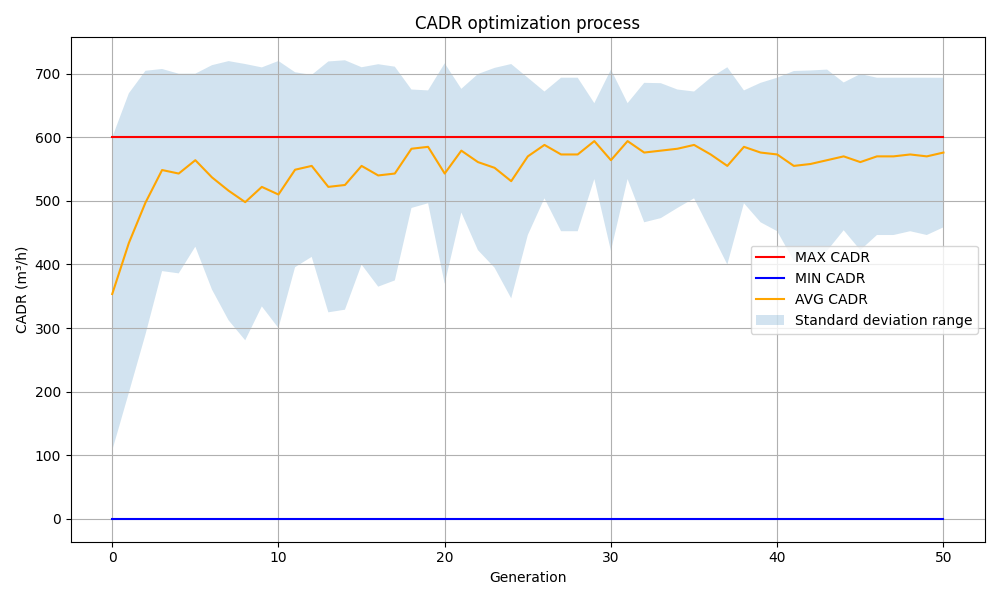
\includegraphics[width=10cm]{q2_CADR_optimization_process}% 图片相对位置
	\caption{Plot of results for 50 iterations of the genetic algorithm} % 图片标题 
\end{figure}

According to Python and combined with the image analysis can be obtained, the maximum value of CADR is 600${m^3}/h$ , the minimum value of CADR is 0, in order to ensure the results of the operation, here take the average value of CADR 550 ${m^3}/h$ .

The optimal air purifier can be obtained with a radius of 0,12 meters, a height of 1.9 meters, 8 filters, 2 air inlets at the top and 4 air outlets at the end, and a CARD=550 
${m^3}/h$ . Its exterior design is shown in the following figure
\begin{figure}[H]
	\centering
	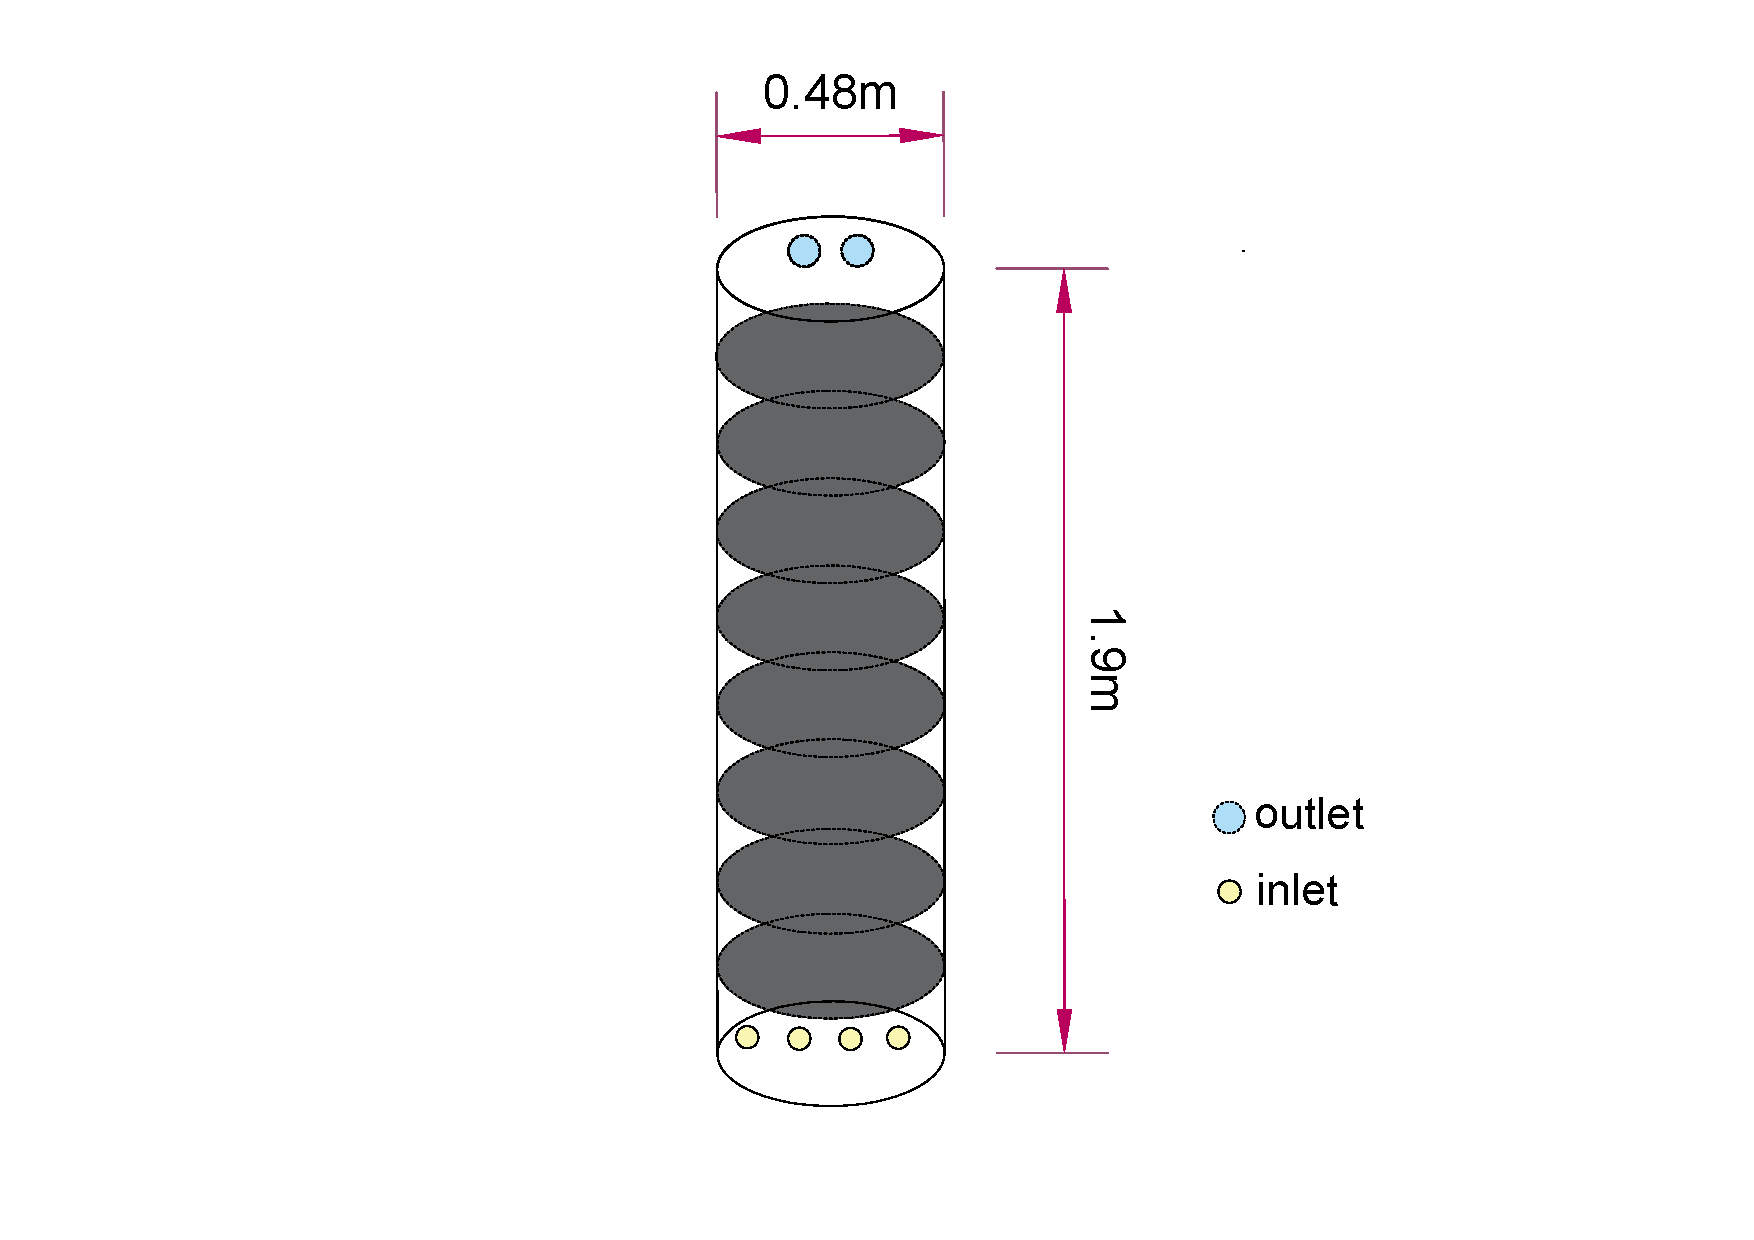
\includegraphics[width=10cm]{jinghuaqi}% 图片相对位置
	\caption{Optimal Air Purifier Exterior Design } % 图片标题 
\end{figure}

It was calculated that the best air purification effect was achieved by placing the air purifier at the position (2.5, 4, 1.5) in the space. The distribution of air purification after 30s, 300s and 600s of operation in the room is shown below.
\begin{figure}[H]
	\centering    
	\subfigure[]{				% 图片1([]内为子图标题)
		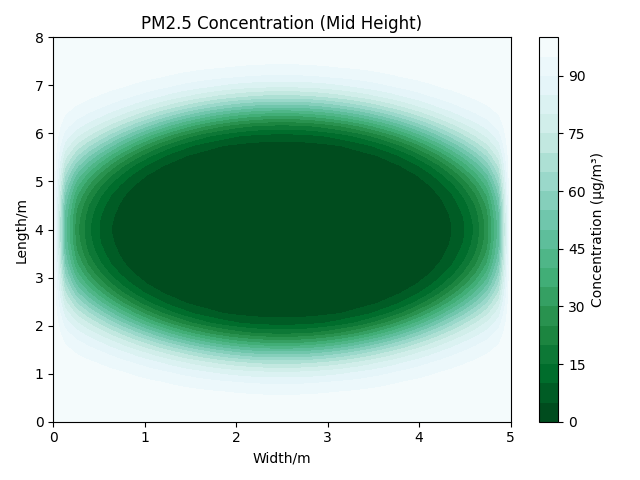
\includegraphics[width=0.3\textwidth]{q2_PM2.5_diff_30.0s}}% 子图1的相对位置
	\subfigure[]{				% 图片2
		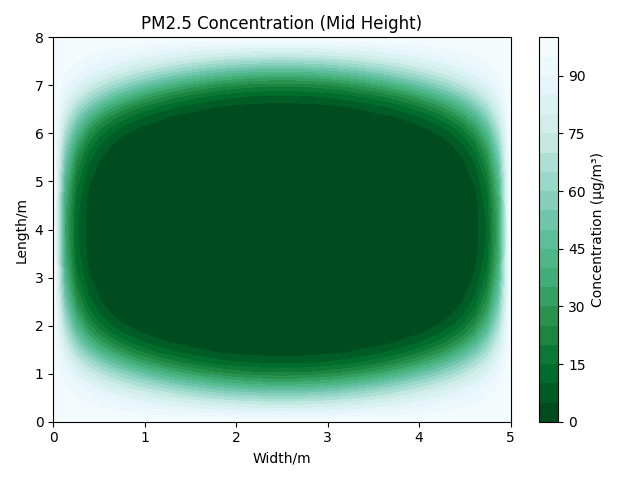
\includegraphics[width=0.3\textwidth]{q2_PM2.5_diff_300.0s}}% 子图2的相对位置
	\subfigure[]{				% 图片2
		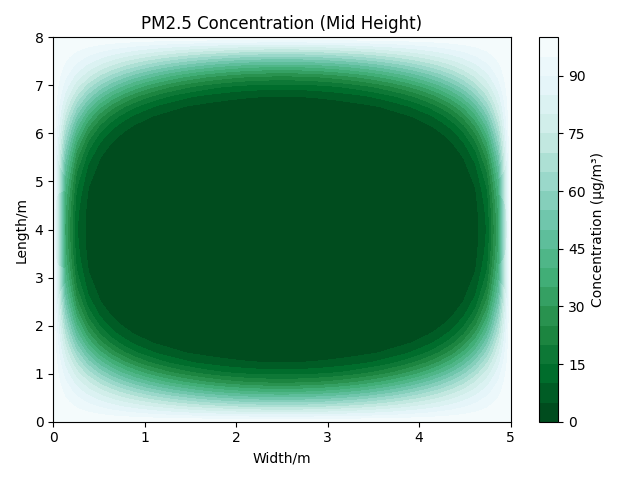
\includegraphics[width=0.3\textwidth]{q2_PM2.5_diff_600.0s}}% 子图3的相对位置
	\caption{Purification after 30, 300 and 600 seconds in a two-dimensional plane}		% 总图标题
\end{figure}
\begin{figure}[H]
	\centering    
	\subfigure[]{				% 图片1([]内为子图标题)
		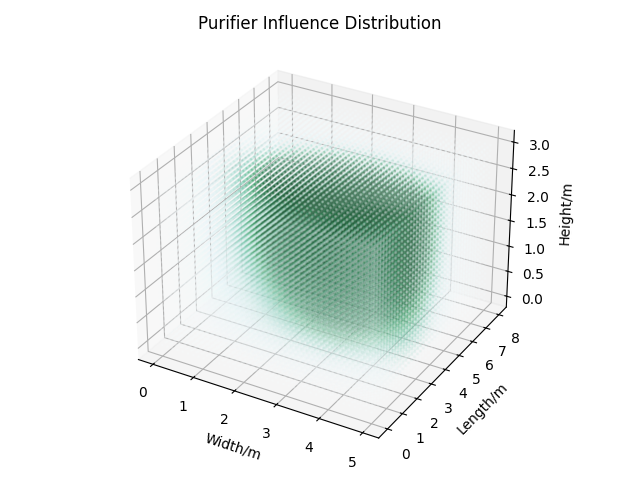
\includegraphics[width=0.3\textwidth]{q2_PM2.5_3-scatter_30.0s}}% 子图1的相对位置
	\subfigure[]{				% 图片2
		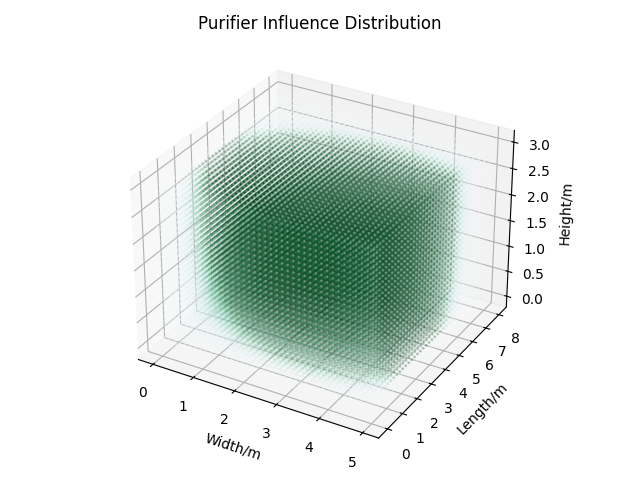
\includegraphics[width=0.3\textwidth]{q2_PM2.5_3-scatter_300.0s}}% 子图2的相对位置
	\subfigure[]{				% 图片2
		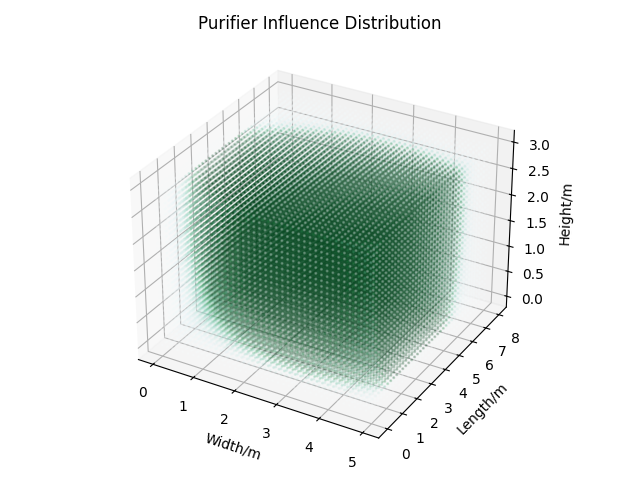
\includegraphics[width=0.3\textwidth]{q2_PM2.5_3-scatter_600.0s}}% 子图3的相对位置
	\caption{Purification after 30, 300 and 600 seconds in a three-dimensional plane}		% 总图标题
\end{figure}

With the passage of time, the indoor two-dimensional air purification range gradually spreads from the location of the air purifier to the surrounding area, and the air purification range in the three-dimensional scattering point gradually spreads from the location of the air purifier to all directions in the space. The desired effect is met.

\subsubsection{Advantages and disadvantages of concentration-diffusion models based on Fick's second law}
\begin{description}
	\item[Strength:] Ability to describe unsteady diffusion processes where concentration varies with time and position according to Fick's second law.
	
	\item[Weakness:] Fick's second law is a macroscopic image-only relational equation that does not address the microscopic processes of atomic motion within a diffusion system and does not fully capture all the physical phenomena of the diffusion process.
\end{description} 

\subsection{Air humidity modeling and solution based on particle swarm algorithm}
Particle swarm algorithm based appearance solving and come to use the finite difference method for simulating the process of humidifier while working in the room.

\subsubsection{ Preparation of air humidity model based on particle swarm algorithm}

The initial humidity at the wall is set to 0.2g/m³ to ensure that the humidity does not appear to penetrate the wall. According to the relevant literature\cite{lgsteamer2024} and market research statistics analysis it is known that the shape of the humidifier is cylindrical as the optimal shape.


\subsubsection{Modeling of air humidity based on particle swarm algorithm}
Due to the slow convergence of genetic algorithm, this question uses particle swarm algorithm to search for the best humidifier design parameters by updating the particles. Its basic flow is shown in the following figure
\begin{figure}[H]
	\centering
	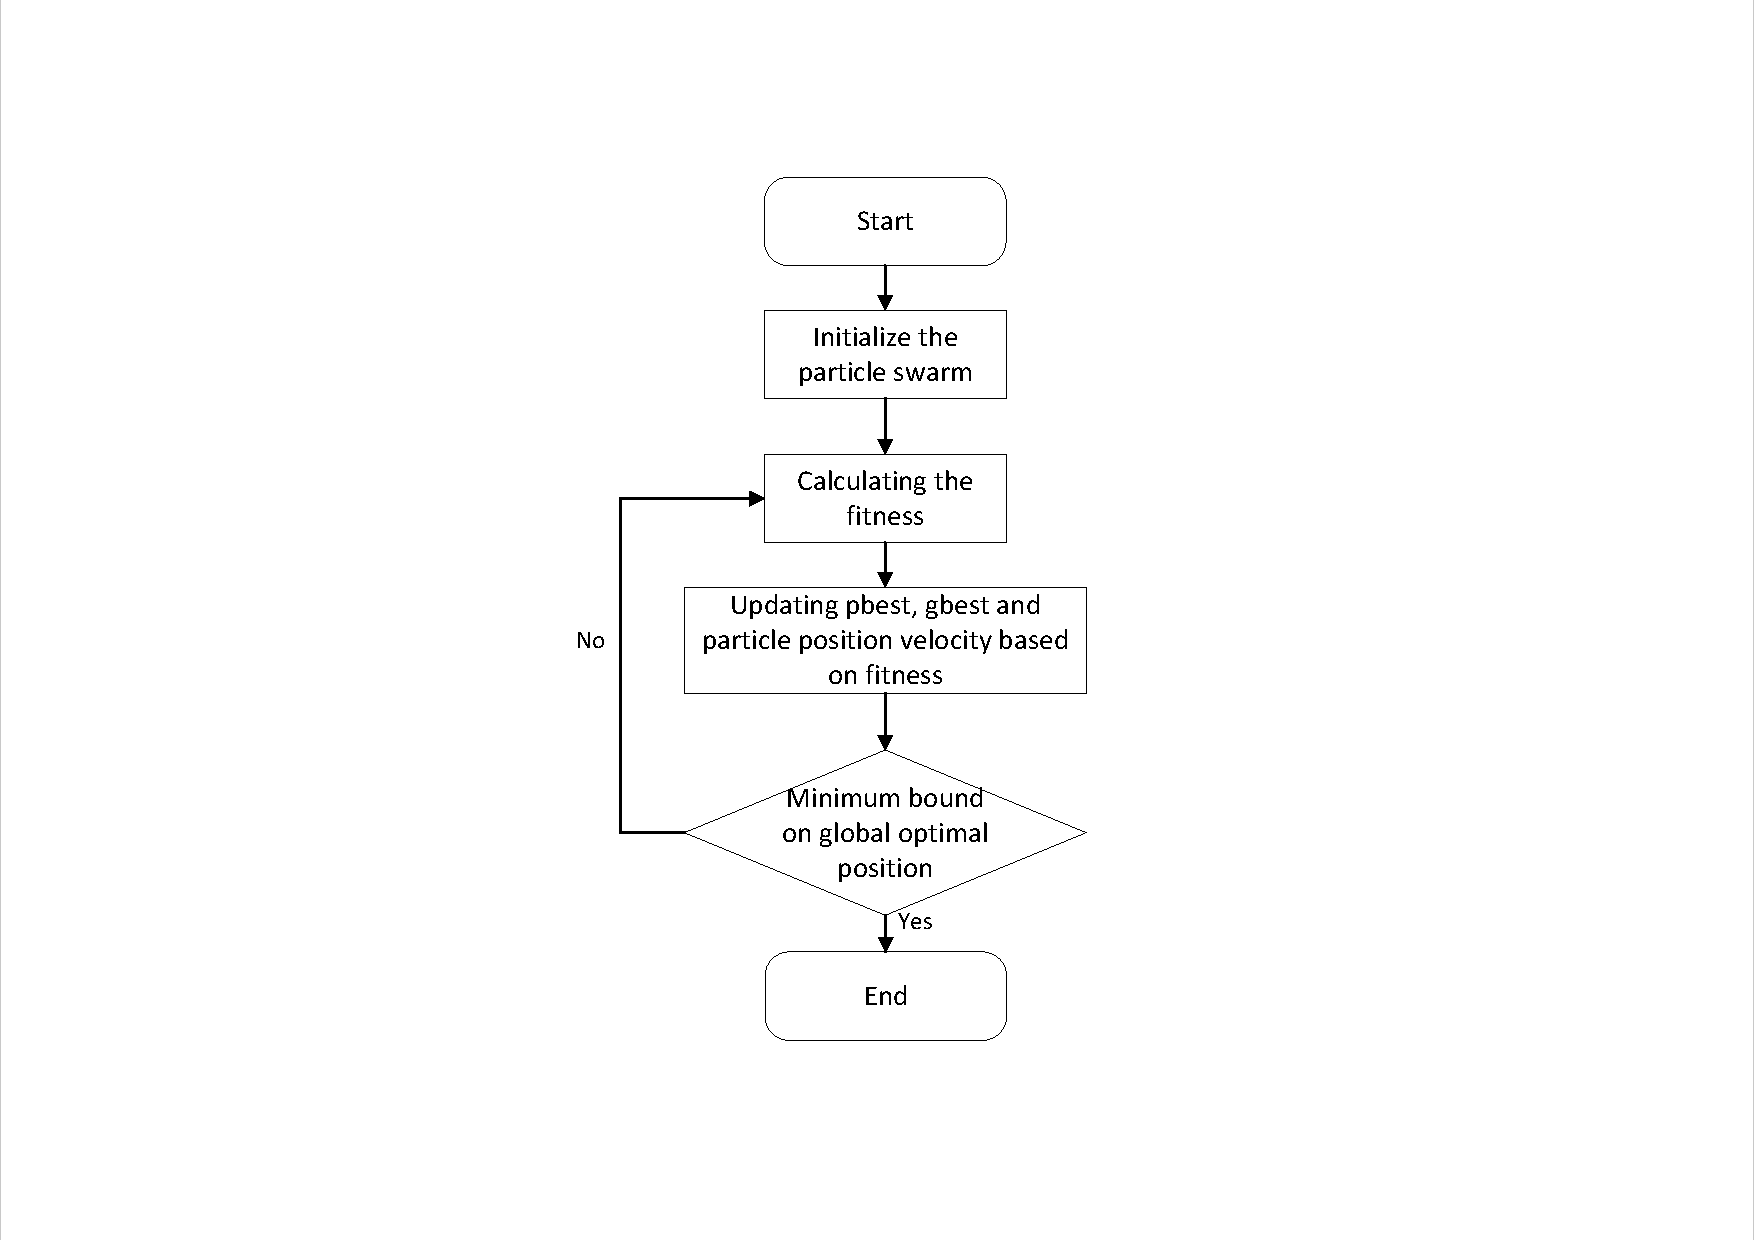
\includegraphics[width=10cm]{PSO}% 图片相对位置
	\caption{Particle swarm algorithm process diagram} % 图片标题 
\end{figure}
The particle swarm is initialized first, and each particle represents a humidifier design whose fitness is evaluated by the humidity effect of the humidifier design, with the goal of maximizing the humidity effect.
The formula for the humidity effect is as follows:
\begin{equation}
	\text{Humidity Effect} = -(2\pi rh) \times \text{Air Velocity} \times \text{Target Humidity Difference}
\end{equation}
In each iteration, the particles are adjusted according to their current position and velocity and updated by the influence of neighboring particles to achieve the air target humidity of 0.6 g/m³. The equation for updating the position of the particle is as follows:
\begin{equation}
	v_i(t+1) = w(X, Y, Z) \cdot v_i(t) + c_1 \cdot r_1 \cdot (pbest_i - x_i(t)) + c_2 \cdot r_2 \cdot (gbest - x_i(t))
\end{equation}

\begin{equation}
	x_i(t+1) = x_i(t) + v_i(t+1)
\end{equation}

Where, is the velocity of the particle in each iteration, is the position of the particle, is the optimal position of a single particle, is the optimal position of the whole particle, is the inertia weight, and are the acceleration constants, and and are random numbers in the range of [0,1].

After several iterations, the optimal exterior size of the humidifier can be derived.

The optimal humidifier parameters obtained above were substituted into the simulation of the indoor humidification process. Within a single time step , the modification process is also investigated using Fick's second law. The humidity field is updated according to the influence of the humidifier and the process of humidity diffusion. The humidity diffusion is calculated by the Laplace operator and the update equation of the humidity field is given by
\begin{equation}
	H_{i,j,k}^{n+1} = H_{i,j,k}^{n} + \Delta t \cdot D \cdot \nabla^2 C
\end{equation}

where D is the diffusion coefficient of humidity.

\subsubsection{Particle Swarm Algorithm Based Solving of Air Humidity Models}
The initial particle swarm is set to 50, and the action radius of the humidifier is 1. The 50 iterations of the particles obtained by the particle swarm algorithm are shown in the figure below.

\begin{figure}[H]
	\centering
	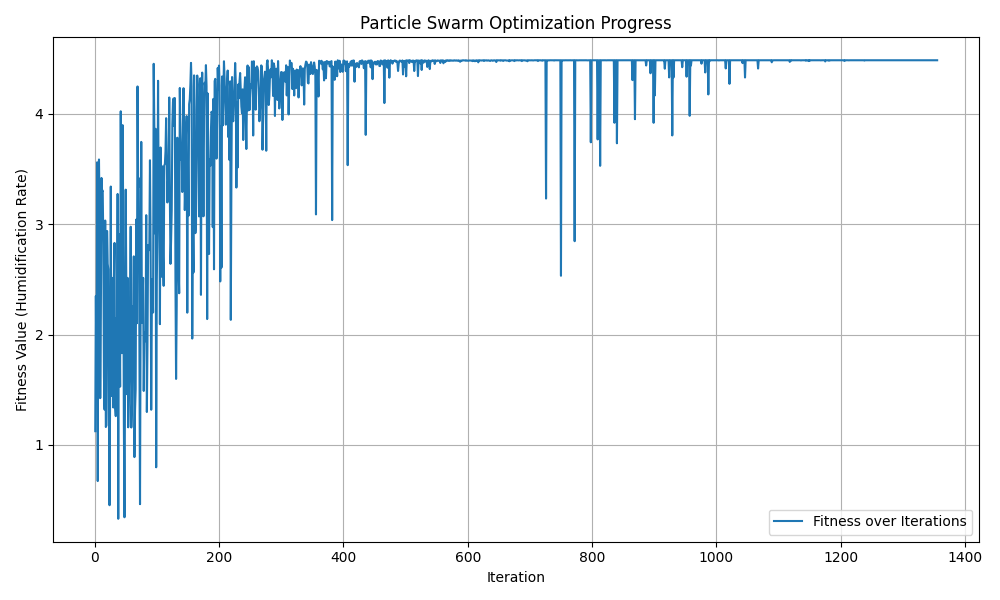
\includegraphics[width=10cm]{q3_weet_pso}% 图片相对位置
	\caption{Particle swarm algorithm after 50 iterations} % 图片标题 
\end{figure}



The optimal solution is calculated and simulated by Python with a humidifier height of 1m, a radius of 0.18m, and a humidification rate of 4.48. The design diagram is shown below
\begin{figure}[H]
	\centering
	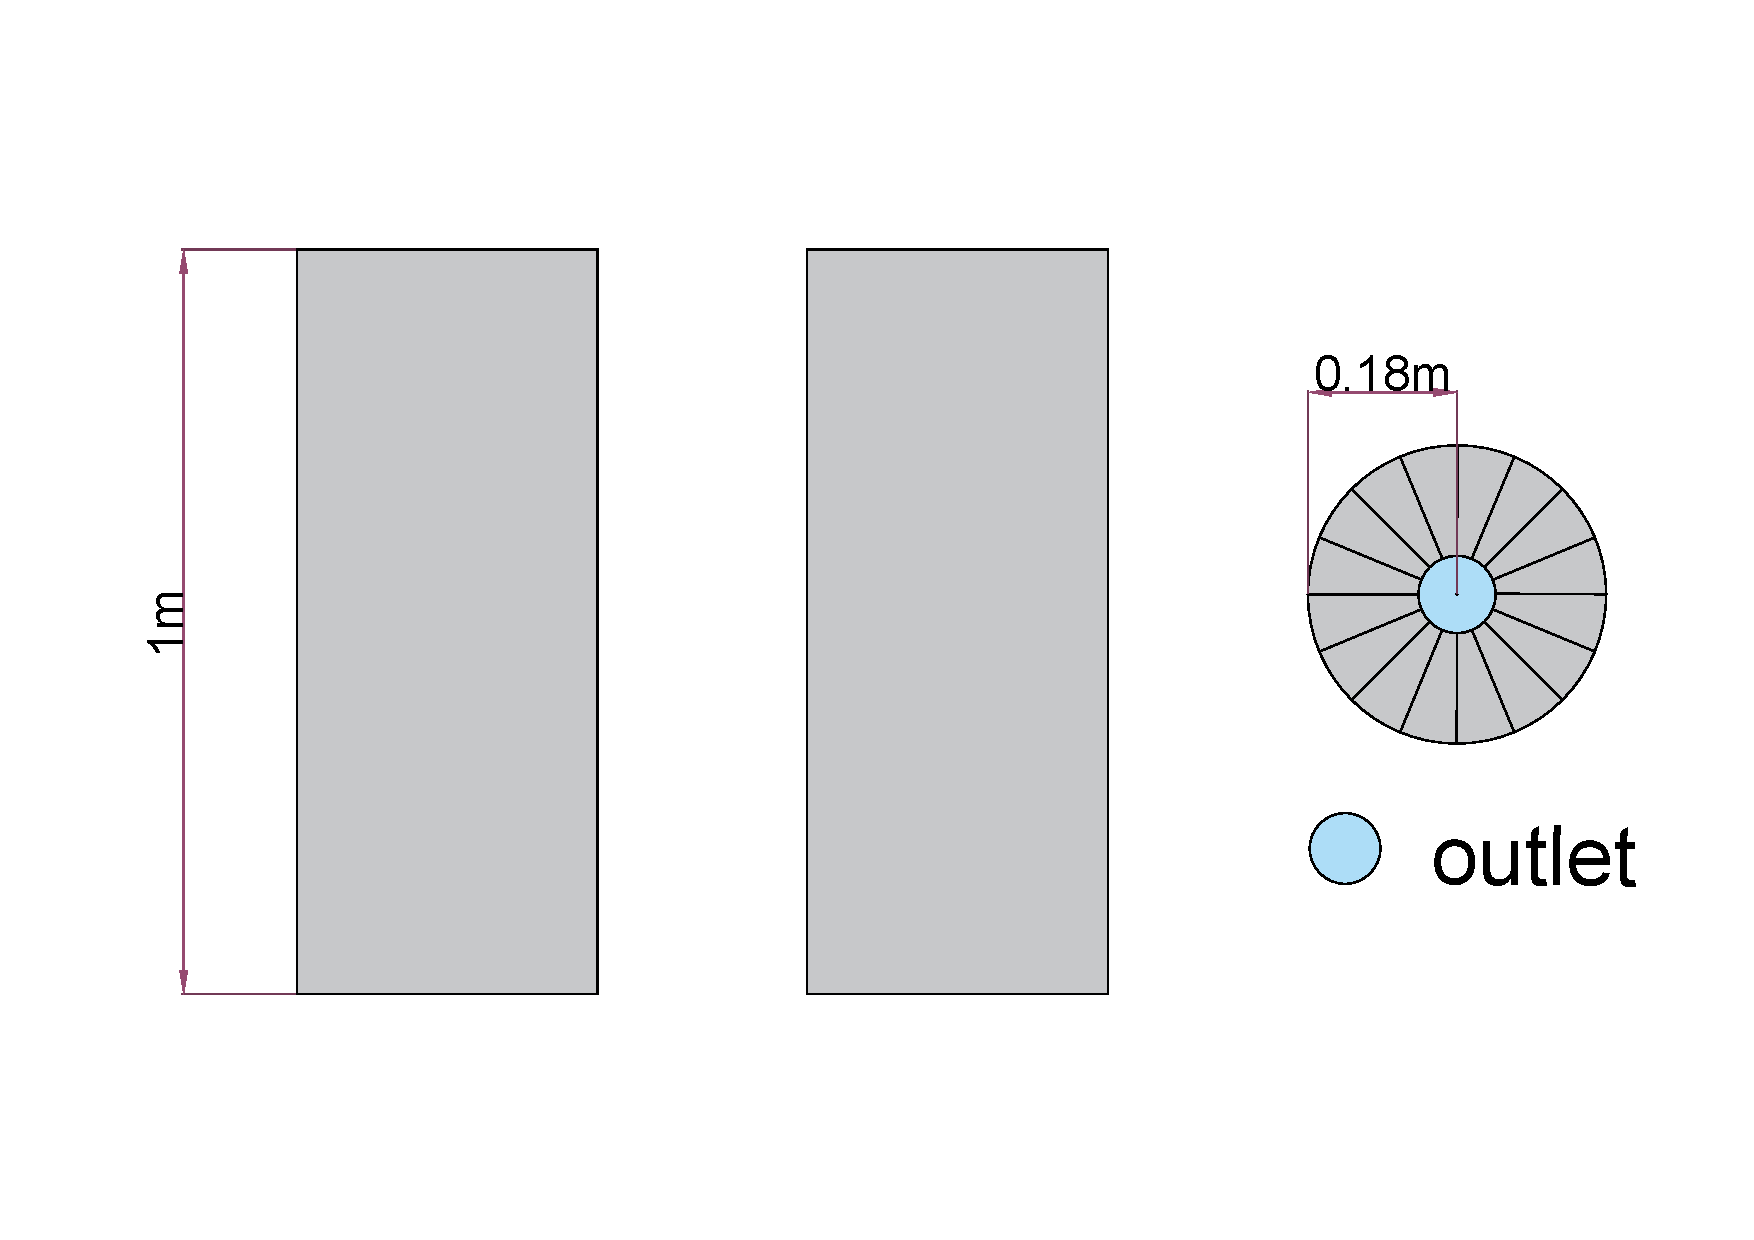
\includegraphics[width=10cm]{jiashiqi}% 图片相对位置
	\caption{Optimal humidifier design} % 图片标题 
\end{figure}



Set the time step and set the target humidity to 0.6 g/m³. The finite difference method similar to the problem class is used to simulate the diffusion process of humidity from high concentration to low concentration. The humidity field distribution after 30s, 300s and 600s of humidity field simulation is shown below.
\begin{figure}[H]
	\centering    
	\subfigure[]{				% 图片1([]内为子图标题)
		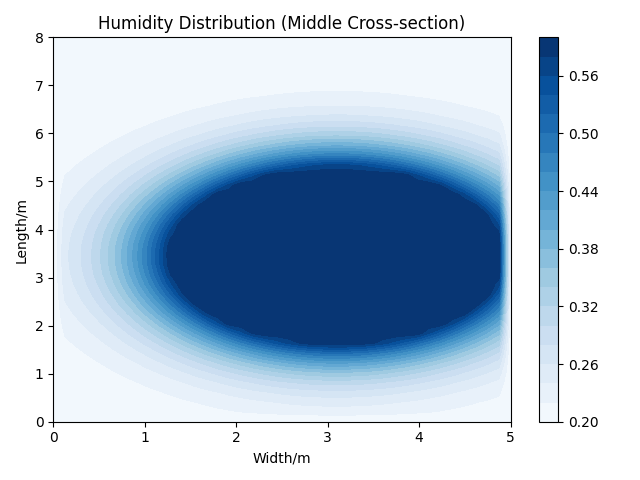
\includegraphics[width=0.3\textwidth]{q3_humidity_diff_30.0s}}% 子图1的相对位置
	\subfigure[]{				% 图片2
		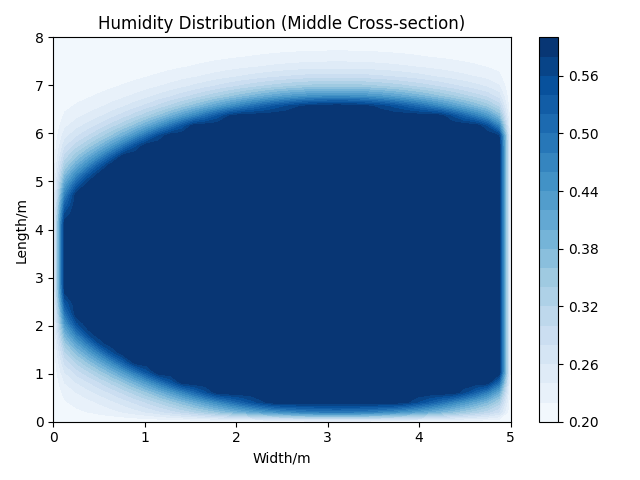
\includegraphics[width=0.3\textwidth]{q3_humidity_diff_300.0s}}% 子图2的相对位置
	\subfigure[]{				% 图片2
		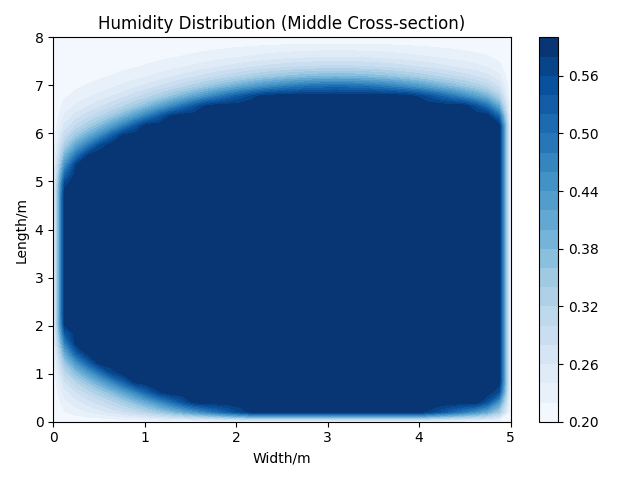
\includegraphics[width=0.3\textwidth]{q3_humidity_diff_600.0s}}% 子图3的相对位置
	\caption{Humidification effect after 30, 300 and 600 seconds in 2D plane}		% 总图标题
\end{figure}
\begin{figure}[H]
	\centering    
	\subfigure[]{				% 图片1([]内为子图标题)
		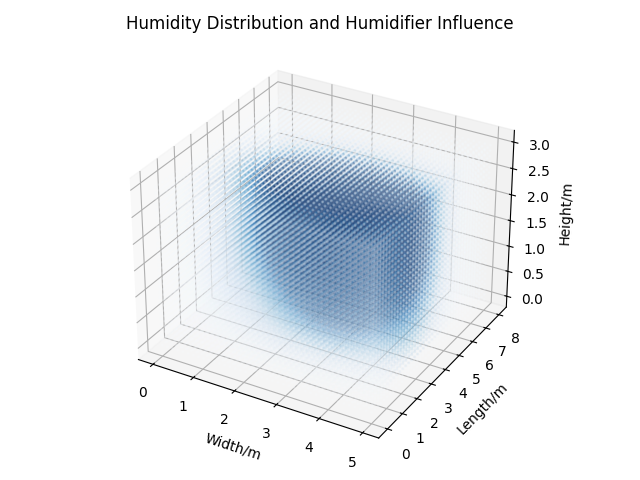
\includegraphics[width=0.3\textwidth]{q3_humidity_scatter_30.0s}}% 子图1的相对位置
	\subfigure[]{				% 图片2
		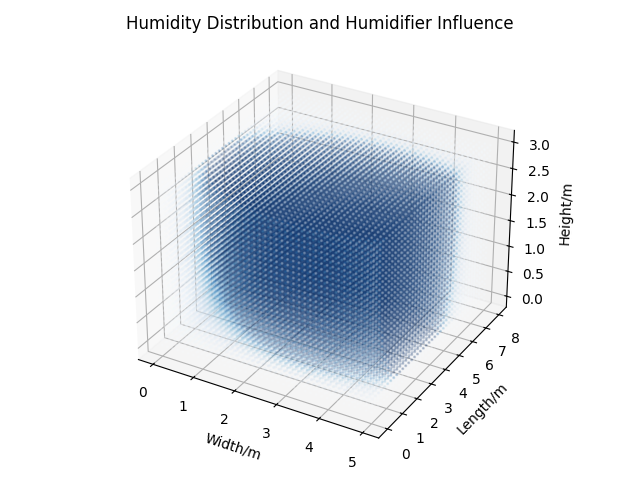
\includegraphics[width=0.3\textwidth]{q3_humidity_scatter_300.0s}}% 子图2的相对位置
	\subfigure[]{				% 图片2
		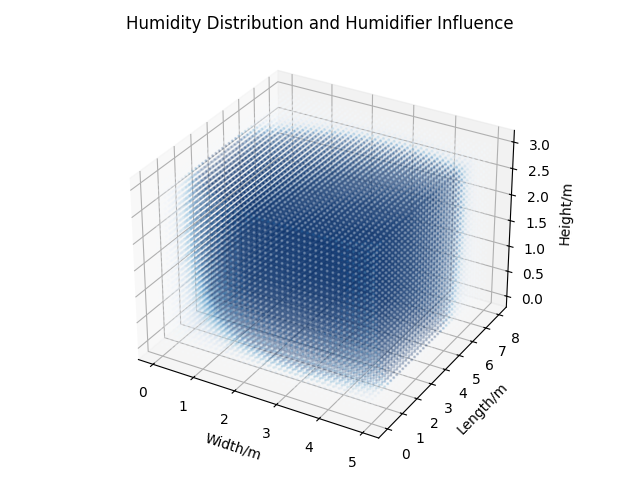
\includegraphics[width=0.3\textwidth]{q3_humidity_scatter_600.0s}}% 子图3的相对位置
	\caption{Humidification effect after 30, 300 and 600 seconds in 3D plane}		% 总图标题
\end{figure}




Over time, the humidity in the indoor two-dimensional humidity field gradually spreads from the humidifier's location to the surrounding area, and the humidity in the three-dimensional scattering point gradually spreads from the humidifier's location to all directions within the space. Some of the indoor time to humidity percentage and average humidity data are shown in the table below.

\begin{table}
	\centering
	\caption{Partial time vs. humidity percentage and average humidity data table} % 表格标题
	\label{tab:partial_time_vs_humidity} % 表格标签,已简化
	\begin{tabular}{ccc} 
		\hline
		Time & Humidity percentage & Average humidity unit \\ 
		\hline
		30s  & 17.85\%             & 0.33                  \\
		300s & 53.19\%             & 0.45                  \\
		600s & 60.79\%             & 0.48                  \\
		\hline
	\end{tabular}
\end{table}

\subsubsection{Strength and Weakness}

\begin{description}
	\item[Strength:]Ability to search over a large range and avoid entering local optimal solutions.Fast convergence, can quickly find a better solution
	\item[Weakness:]  May result in a less refined search capability due to insufficient particle swarm diversity.
\end{description}
\subsection{Combinatorial optimization model building and solution based on genetic algorithm}
Optimization of three-in-one products using genetic algorithms to obtain optimal appearance dimensions.

\subsubsection{Preparation of Combinatorial Optimization Model Based on Genetic Algorithm}

Placing the humidifier above the vertical air conditioner will accelerate the diffusion of the water mist in the humidifier by utilizing the wind blowing from the air conditioner, resulting in a more uniform indoor humidity. Therefore, it was chosen to place the humidifier above the vertical air conditioner during the design.
In the choice of shape, since the first three questions are in cylindrical shape, the cylindrical shape is directly used in the setting of the 3-in-1 product.


\subsubsection{Establishment of Combinatorial Optimization Model Based on Genetic Algorithm}
The optimal air conditioner size can be derived according to the genetic algorithm. The basic process is shown below.

For the design of three-in-one products, genetic algorithms can be used to simultaneously optimize multiple design parameters for all three devices.

The optimization objective is to minimize the temperature deviation and maximize the humidity control while satisfying the volume constraints. The constraints consider the radius, number of inlet and outlet ports, and location of the air conditioner, radius, number of filter layers, number of inlet and outlet ports, and location of the purifier, and radius, number of inlet and outlet ports, and location of the humidifier. Optimization is done by genetic algorithm.

Similar to the genetic algorithm described above, the population size is initialized first. In considering the fitness function, the temperature deviation, humidity control effect and device size are taken into account.

For temperature deviation
\begin{equation}
	\text{Temperature Deviation} = \sum \left| T_{\text{new}}(i, j, k) - T_{\text{target}} \right|
\end{equation}
For temperature control
\begin{equation}
	\text{Humidity Deviation} = \sum \left| H_{\text{new}}(i, j, k) - H_{\text{target}} \right|
\end{equation}
For volume limitation
\begin{equation}
	{{V}_{total}}={{V}_{ac}}+{{V}_{purifier}}+{{V}_{humidifier}}\le {{P}_{\max }}
\end{equation}

The final fitness function can be expressed by weighting and combining all of the above terms.
\begin{equation}
	\text{Fitness} = w_1 \cdot \text{Temperature Deviation} + w_2 \cdot \text{Humidity}
\end{equation}

where w1,w2,w3 are the weighting coefficients.

After that the selection operation uses tournament selection to enter the screened individuals into the crossover and mutation operation. After that it is chosen whether to enter the selection operation or not according to the optimization objective. The optimal size result can be obtained after performing several iterations.

\subsubsection{Genetic Algorithm Based Combinatorial Optimization Model Solving}
Let the initial population size be 100, and simulate the genetic algorithm through Python after 50 iterations image as follows.

\begin{figure}[H]
	\centering
	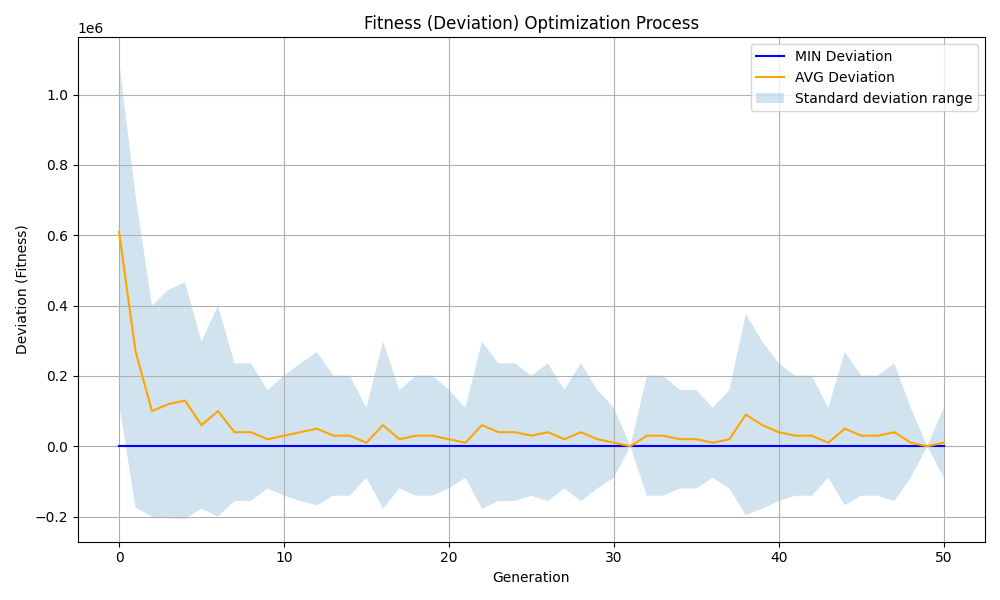
\includegraphics[width=8cm]{q4_fitness_optimization_process}% 图片相对位置
	\caption{Plot of results for 50 iterations of the genetic algorithm} % 图片标题 
\end{figure}

The optimal solution is 0.2884 m height for the air conditioner, 0.0961 m height for the purifier, 0.0961 m height for the humidifier, 0.4807 m height for the total equipment, and 0.0944 m³ total volume. Its shape design scheme is shown below.
\begin{figure}[H]
	\centering    
	\subfigure[]{				% 图片1([]内为子图标题)
		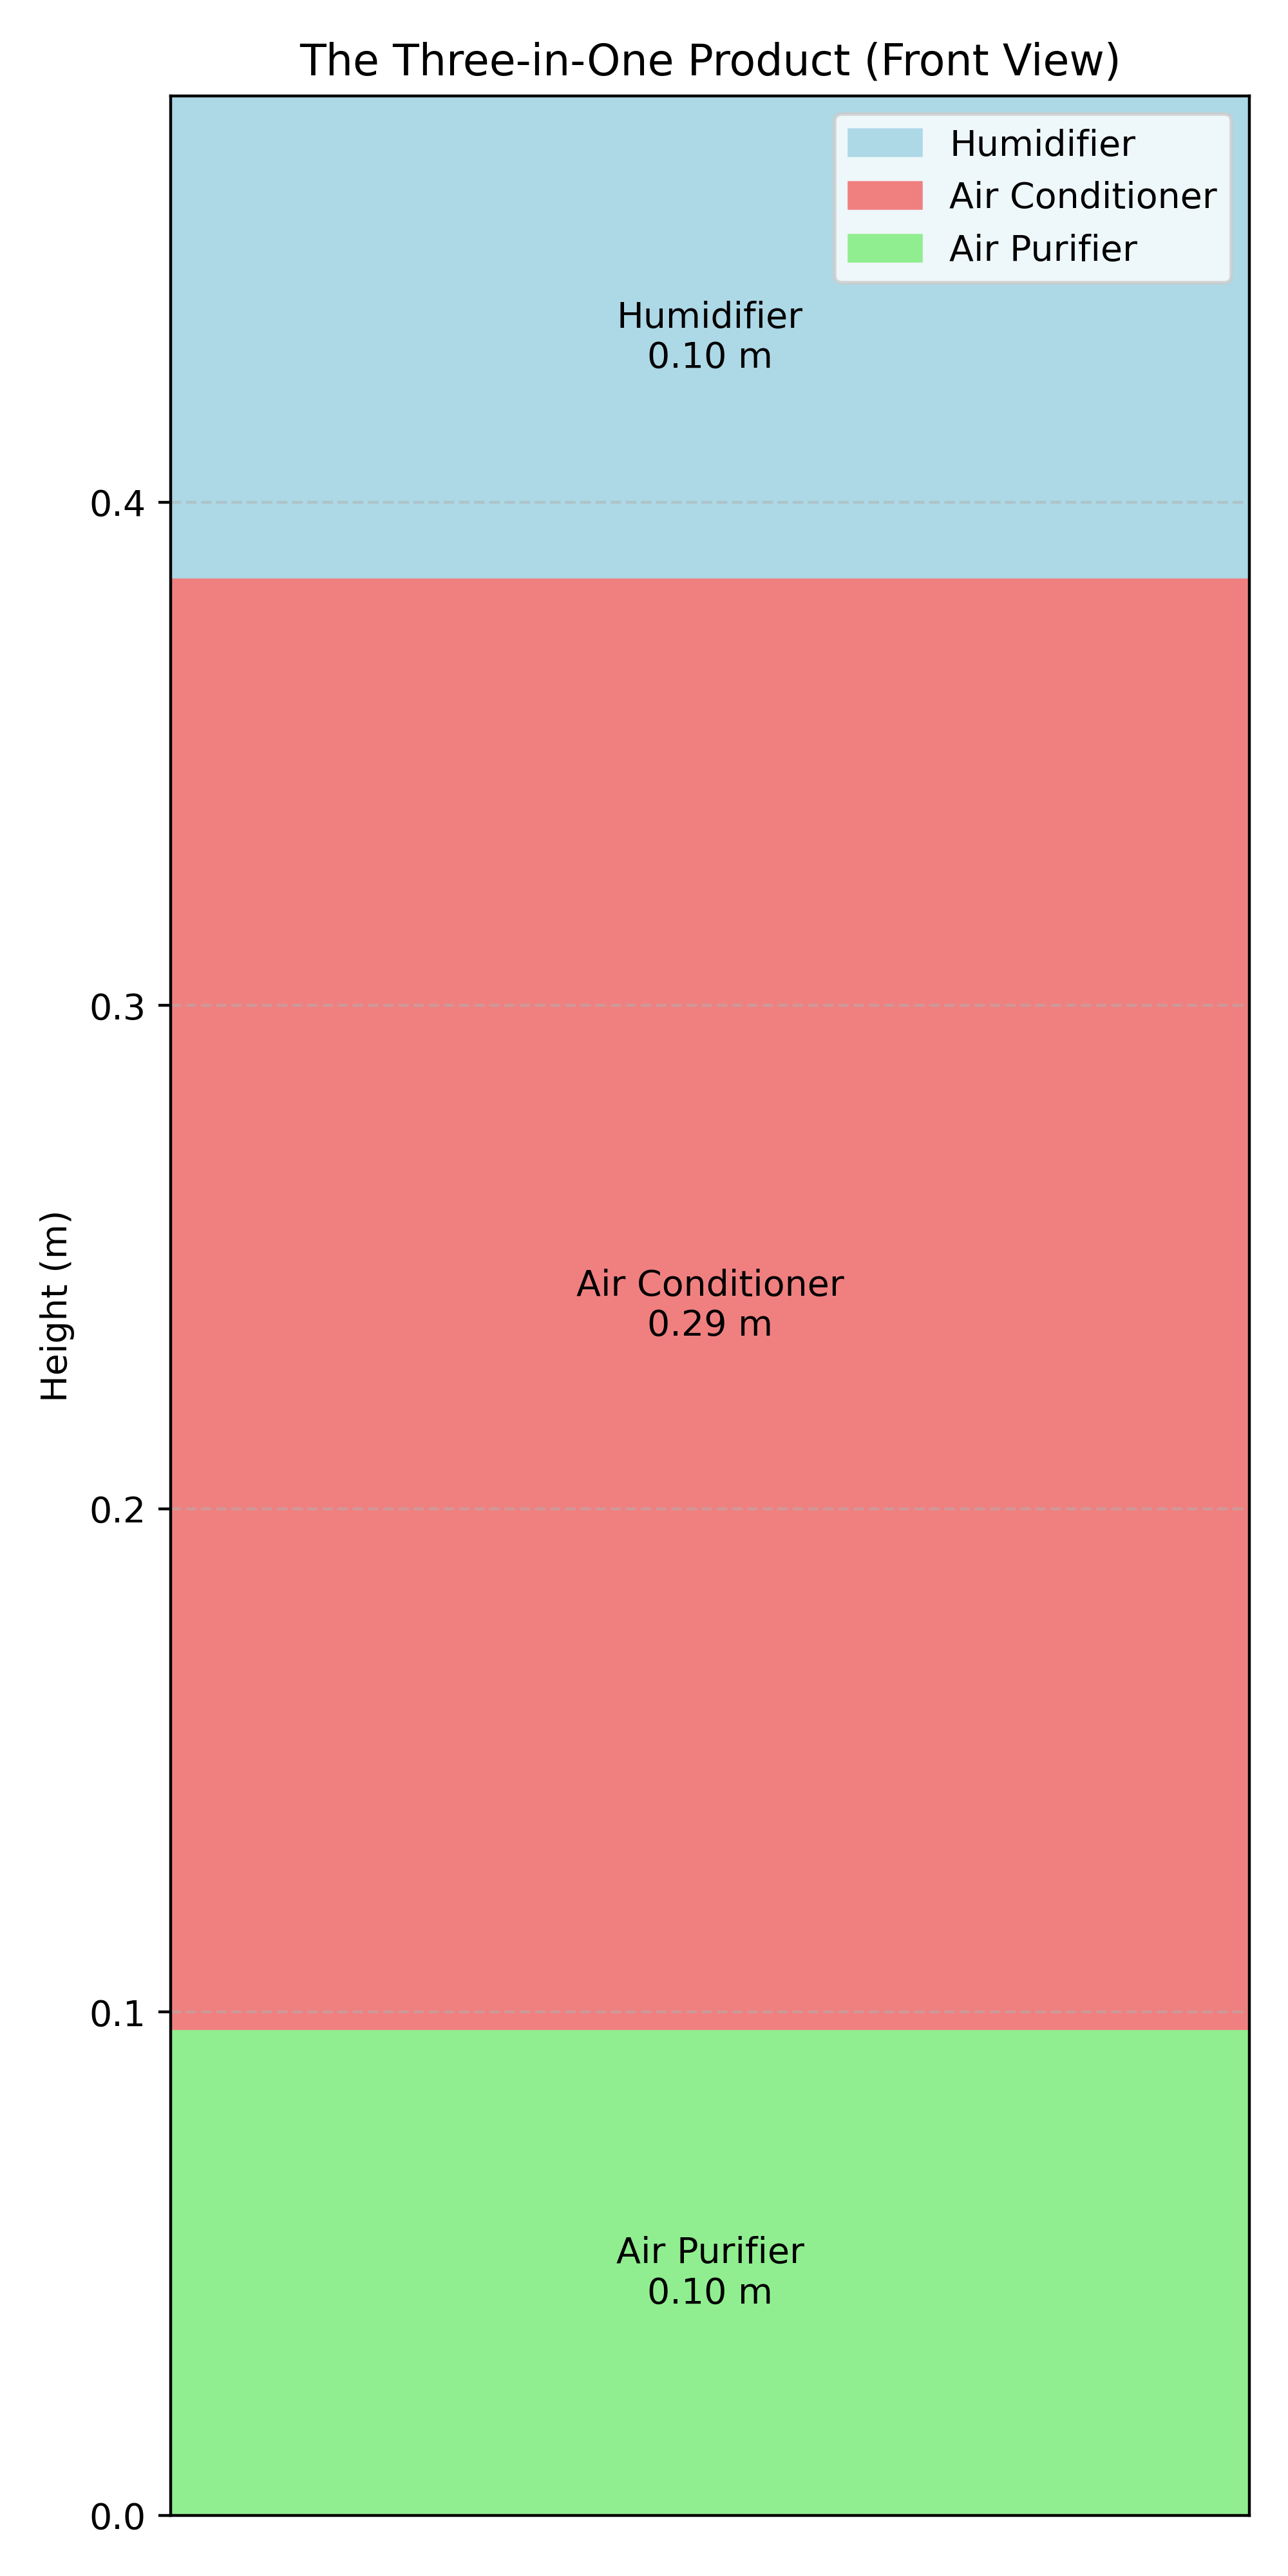
\includegraphics[width=0.2\textwidth]{q4_The_three_in_one_product}}% 子图1的相对位置
	\subfigure[]{				% 图片2
		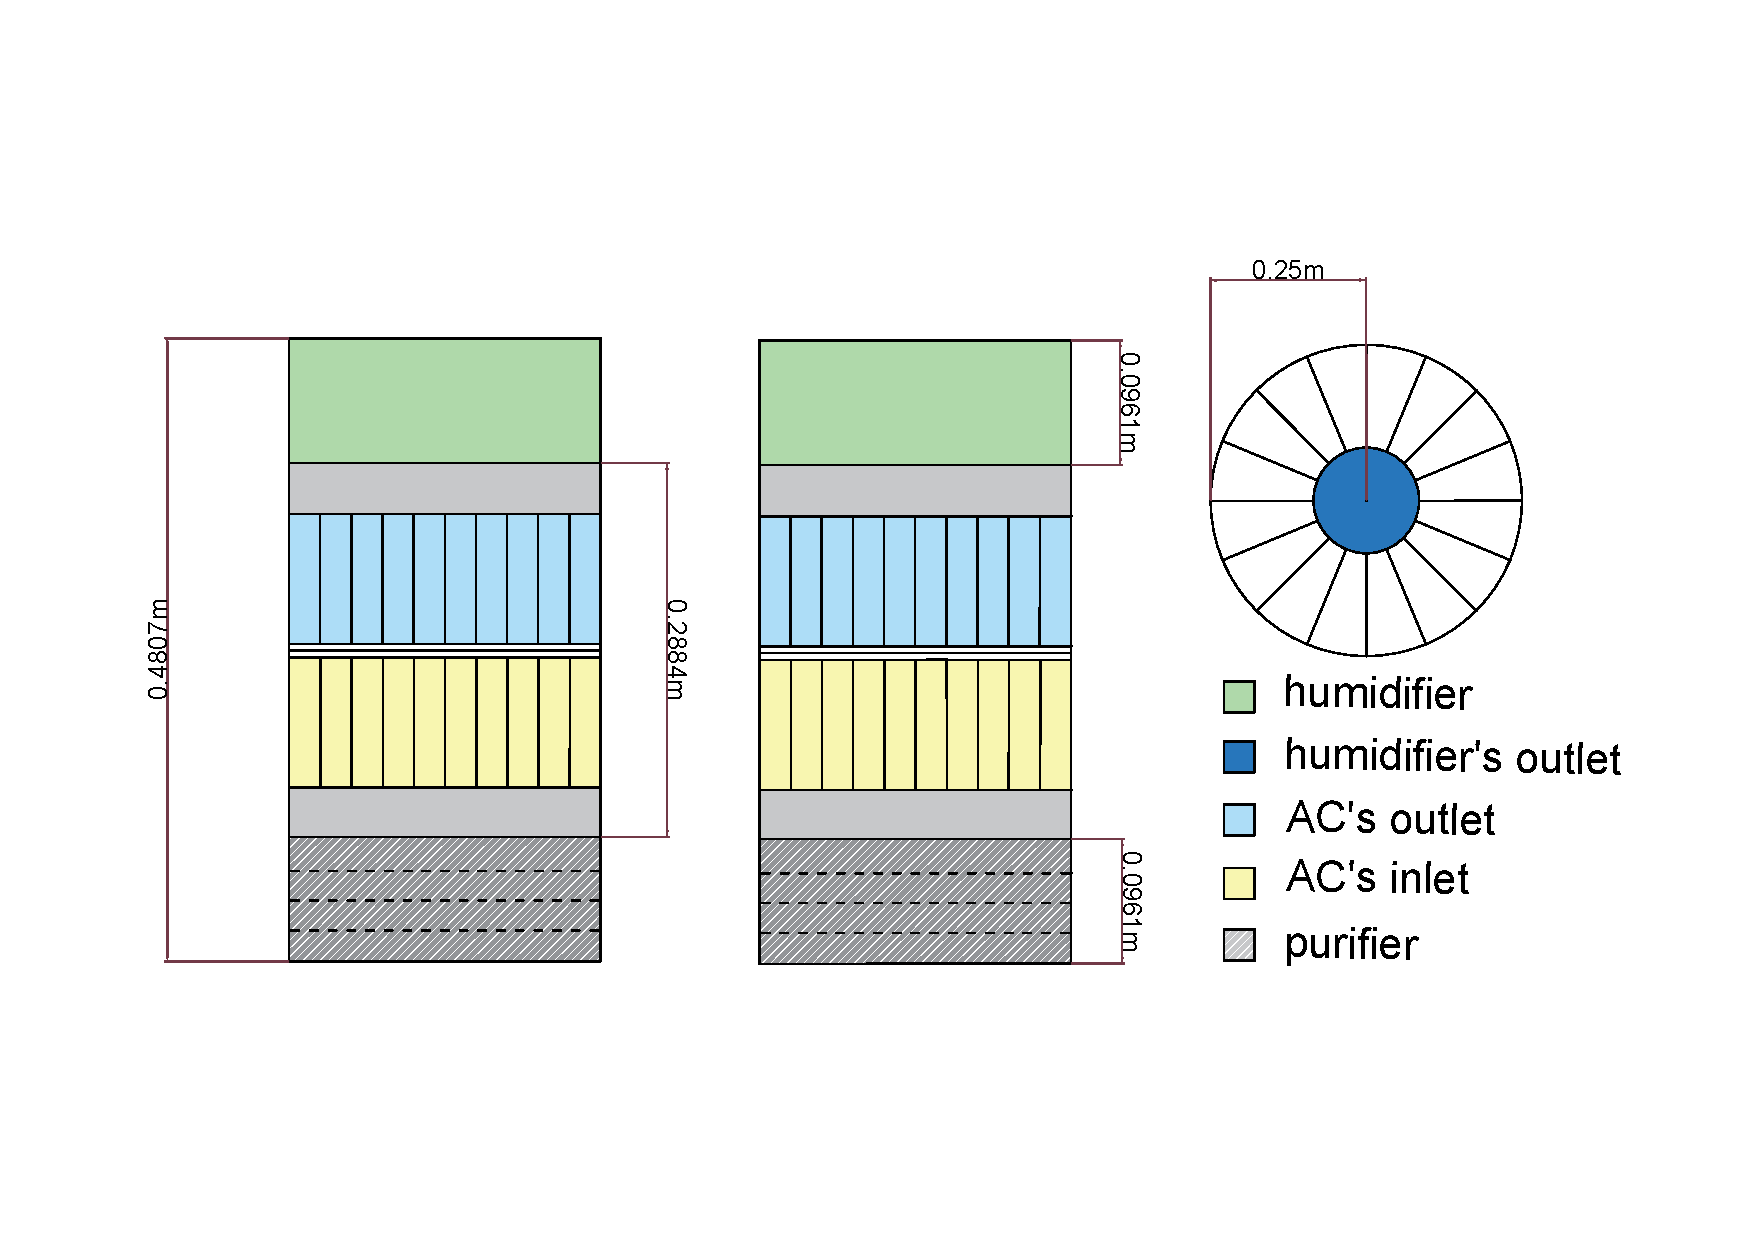
\includegraphics[width=0.5\textwidth]{three-one}}% 子图2的相对位置
	\caption{Optimal design diagram for 3-in-1 products}		% 总图标题
\end{figure}

\subsubsection{Strength and Weakness}

\begin{description}
	\item[Strength:]  Higher flexibility to consider multiple objectives and meet the needs of different stakeholders
	\item[Weakness:]  Slow convergence in the face of large computational volumes.
\end{description}
\subsection{Evaluation and Outlook}
Optimization of three-in-one products using genetic algorithms to obtain optimal appearance dimensions.
\subsubsection{Evaluation}
The genetic algorithm used in this paper has a population size of 100 and an iteration number of 50, and according to the image analysis related to the above content, it has good convergence, so the results obtained are the best results. The particle swarm algorithm population size is 50, the number of iterations is 50, according to the above content related image analysis can be obtained, has good convergence, so the results obtained are the best results.
\subsubsection{Outlook}
The model provided in this question needs to consider the performance and adaptability under different conditions in the actual deployment situation, to ensure that it can still run stably in the changing environment.


%参考文献
\begin{thebibliography}{9}%宽度9
\bibitem{olszewska2024}
Olszewska, P. K., Pinkos, J., Borkowski, D., \& Jablonski, M. 
Modeling the Geometry and Filter Composite of the Air Cleaner. 
\textit{Materials}, \textbf{17}(20), 4969, 2024.

\bibitem{sadrizadeh2022indoor}
Sadrizadeh, S., Yao, R., Yuan, F., Awbi, H., Bahnfleth, W., Bi, Y., Cao, G., Croitoru, C., de Dear, R., Haghighat, F., \& others. 
Indoor air quality and health in schools: A critical review for developing the roadmap for the future school environment. 
\textit{Journal of Building Engineering}, \textbf{57}, 104908, 2022. 
\texttt{https://doi.org/10.1016/j.jobe.2021.104908}.

\bibitem{zhu2002concentration}
Zhu, Y., Hinds, W. C., Kim, S., \& Sioutas, C. 
Concentration and size distribution of ultrafine particles near a major highway. 
\textit{Journal of the Air \& Waste Management Association}, \textbf{52}(9), 1032--1042, 2002. 
\texttt{https://doi.org/10.1080/10473289.2002.10470842}.

\bibitem{lgsteamer2024}
LG Electronics Inc. 
\textit{LG Steamer (H–63HSW)}. 
Red Dot Design Award, 2024. 
\texttt{https://www.red-dot.org/project/lg-steamer-h-63hsw-31432}.

\end{thebibliography}

\newpage
%附录

\section{Appendix}
\begin{lstlisting}[language=python,caption={The code path for question1 in Python}]
	\question1\q1_Re_num.py
	\question1\q1_position_ga.py
	\question1\q1_air_diffusivity.py
	\question1\q1_Initial_state_code.py
	\question1\q1_diffusion_times.py
	\question1\q1_lines.py
 \end{lstlisting}
\begin{lstlisting}[language=python,caption={The code path for question2 in Python}]
	\question2\q2_cadr_design.py
	\question2\q2_picture_design.py
	\question2\q2_situation.py
 \end{lstlisting}
\begin{lstlisting}[language=python,caption={The code path for question3 in Python}]
	\question2\q3_airhum_alpha.py
	\question2\q3_weet_pso.py
	\question2\q3_hum_situation.py
\end{lstlisting}
\begin{lstlisting}[language=python,caption={The code path for question4 in Python}]
	\question4\q4_design.py
\end{lstlisting}
\begin{lstlisting}[language=python,caption={The original image path}]
	\figures\
\end{lstlisting}


\end{document} 